\documentclass [PhD] {uclathes}

% \newcommand{\hvecf}{{\mathbf h}}
\newcommand{\bvecf}{{\mathbf b}}
\newcommand{\pvecf}{{\mathbf p}}
\newcommand{\kvecf}{{\mathbf k}}
\newcommand{\wvecf}{{\mathbf w}}
\newcommand{\nvecf}{{\mathbf n}}
\newcommand{\qvecf}{{\mathbf q}}
\newcommand{\yvecf}{{\mathbf y}}
\newcommand{\cvecf}{{\mathbf c}}
\newcommand{\zvecf}{{\mathbf z}}
\newcommand{\uvecf}{{\mathbf u}}
\newcommand{\vvecf}{{\mathbf v}}
\newcommand{\mvecf}{{\mathbf m}}
\newcommand{\avecf}{{\mathbf a}}
\newcommand{\lvecf}{{\mathbf l}}
\newcommand{\xvecf}{{\mathbf x}}
\newcommand{\Gvecf}{{\mathbf G}}
\newcommand{\dvecf}{{\mathbf d}}
\newcommand{\evecf}{{\mathbf e}}
\newcommand{\tvecf}{{\mathbf t}}
\newcommand{\svecf}{{\mathbf s}}
\newcommand{\rvecf}{{\mathbf r}}
\newcommand{\gvecf}{{\mathbf g}}
%\newcommand{\hvec}{{\mathrm h}}
%\newcommand{\bvec}{{\mathrm b}}
%\newcommand{\pvec}{{\mathrm p}}
%\newcommand{\kvec}{{\mathrm k}}
%\newcommand{\wvec}{{\mathrm w}}
%\newcommand{\nvec}{{\mathrm n}}
%\newcommand{\qvec}{{\mathrm q}}
%\newcommand{\yvec}{{\mathrm y}}
%\newcommand{\cvec}{{\mathrm c}}
%\newcommand{\zvec}{{\mathrm z}}
%\newcommand{\uvec}{{\mathrm u}}
%\newcommand{\vvec}{{\mathrm v}}
%\newcommand{\mvec}{{\mathrm m}}
%\newcommand{\avec}{{\mathrm a}}
%\newcommand{\lvec}{{\mathrm l}}
%\newcommand{\xvec}{{\mathrm x}}
%\newcommand{\dvec}{{\mathrm d}}
%\newcommand{\evec}{{\mathrm e}}
%\newcommand{\tvec}{{\mathrm t}}
%\newcommand{\svec}{{\mathrm s}}
%\newcommand{\rvec}{{\mathrm r}}
%\newcommand{\gvec}{{\mathrm g}}

\newcommand{\hvec}{{h}}
\newcommand{\bvec}{{b}}
\newcommand{\pvec}{{p}}
\newcommand{\kvec}{{k}}
\newcommand{\wvec}{{w}}
\newcommand{\nvec}{{n}}
\newcommand{\qvec}{{q}}
\newcommand{\yvec}{{y}}
\newcommand{\cvec}{{c}}
\newcommand{\zvec}{{z}}
\newcommand{\uvec}{{u}}
\newcommand{\vvec}{{v}}
\newcommand{\mvec}{{m}}
\newcommand{\avec}{{a}}
\newcommand{\lvec}{{l}}
\newcommand{\xvec}{{x}}
\newcommand{\dvec}{{d}}
\newcommand{\evec}{{e}}
\newcommand{\tvec}{{t}}
\newcommand{\svec}{{s}}
\newcommand{\rvec}{{r}}
\newcommand{\gvec}{{g}}
\newcommand{\Gvec}{{\mathrm G}}
\newcommand{\lambdavec}{$$\mbox{\boldmath$\lambda$}$$}
\newcommand{\Thetamat}{{\mathbf \Theta}}
\newcommand{\Phimat}{{\mathbf \Phi}}
\newcommand{\Deltamat}{{\mathbf \Delta}}
\newcommand{\Sigmamat}{{\mathbf \Sigma}}
\newcommand{\Omegamat}{{\mathbf \Omega}}
\newcommand{\Psimat}{{ \Psi}}
\newcommand{\Pimat}{{\mathbf \Pi}}
\newcommand{\Gammamat}{{\mathbf \Gamma }}
\newcommand{\Lambdamat}{{\mathbf \Lambda}}
\newcommand{\epsilonvec}{{\mathbf \epsilon}}
\newcommand{\etavec }{{\mathbf \eta }}
\newcommand{\zeromat }{{\mathbf 0 }}
\newcommand{\Zeromat }{{\mathbf 0 }}
%\newcommand{\log10}{{\log_{10}}}
\newcommand{\Gmat}{{G}}
\newcommand{\Omat}{{O}}
\newcommand{\Mmat}{{M}}
\newcommand{\Lmat}{{L}}
\newcommand{\Emat}{{E}}
\newcommand{\Vmat}{{V}}
\newcommand{\Kmat }{{K}}
\newcommand{\Fmat }{{F}}
\newcommand{\Bmat}{{B}}
\newcommand{\Cmat}{{C}}
\newcommand{\Hmat}{{H}}
\newcommand{\Imat}{{\mathbf I}}
\newcommand{\Dmat}{{D}}
\newcommand{\Qmat}{{Q}}
\newcommand{\Rmat}{{R}}
\newcommand{\Jmat}{{J}}
\newcommand{\Xmat}{{X}}
\newcommand{\Nmat}{{N}}
\newcommand{\Amat}{{A}}
\newcommand{\Ymat}{{Y}}
\newcommand{\Wmat}{{W}}
\newcommand{\Umat}{{U}}
\newcommand{\Tmat}{{T}}
\newcommand{\Smat}{{S}}
\newcommand{\Zmat}{{Z}}
\newcommand{\Pmat}{{P}}
%\newcommand{\Gmat}{{\mathrm G}}
%\newcommand{\Omat}{{\mathrm O}}
%\newcommand{\Mmat}{{\mathrm M}}
%\newcommand{\Lmat}{{\mathrm L}}
%\newcommand{\Emat}{{\mathrm E}}
%\newcommand{\Vmat}{{\mathrm V}}
%\newcommand{\Kmat }{{\mathrm K}}
%\newcommand{\Fmat }{{\mathrm F}}
%\newcommand{\Bmat}{{\mathrm B}}
%\newcommand{\Cmat}{{\mathrm C}}
%\newcommand{\Hmat}{{\mathrm H}}
%\newcommand{\Imat}{{\mathrm I}}
%\newcommand{\Dmat}{{\mathrm D}}
%\newcommand{\Qmat}{{\mathrm Q}}
%\newcommand{\Rmat}{{\mathrm R}}
%\newcommand{\Jmat}{{\mathrm J}}
%\newcommand{\Xmat}{{\mathrm X}}
%\newcommand{\Nmat}{{\mathrm N}}
%\newcommand{\Amat}{{\mathrm A}}
%\newcommand{\Ymat}{{\mathrm Y}}
%\newcommand{\Wmat}{{\mathrm W}}
%\newcommand{\Umat}{{\mathrm U}}
%\newcommand{\Tmat}{{\mathrm T}}
%\newcommand{\Smat}{{\mathrm S}}
%\newcommand{\Zmat}{{\mathrm Z}}
%\newcommand{\Pmat}{{\mathrm P}}
\newcommand{\Gmatf}{{\mathbf G}}
\newcommand{\Omatf}{{\mathbf O}}
\newcommand{\Mmatf}{{\mathbf M}}
\newcommand{\Lmatf}{{\mathbf L}}
\newcommand{\Ematf}{{\mathbf E}}
\newcommand{\Vmatf}{{\mathbf V}}
\newcommand{\Rmatf}{{\mathbf R}}
\newcommand{\Kmatf }{{\mathbf K}}
\newcommand{\Fmatf }{{\mathbf F}}
\newcommand{\Hmatf}{{\mathbf H}}
\newcommand{\Imatf}{{\mathbf I}}
\newcommand{\Dmatf}{{\mathbf D}}
\newcommand{\Qmatf}{{\mathbf Q}}
\newcommand{\Jmatf}{{\mathbf J}}
\newcommand{\Xmatf}{{\mathbf X}}
\newcommand{\Nmatf}{{\mathbf N}}
\newcommand{\Amatf}{{\mathbf A}}
\newcommand{\Ymatf}{{\mathbf Y}}
\newcommand{\Wmatf}{{\mathbf W}}
\newcommand{\Umatf}{{\mathbf U}}
\newcommand{\Tmatf}{{\mathbf T}}
\newcommand{\Smatf}{{\mathbf S}}
\newcommand{\Zmatf}{{\mathbf Z}}
\newcommand{\Pmatf}{{\mathbf P}}
\newcommand{\Bmatf}{{\mathbf B}}
\newcommand{\Cmatf}{{\mathbf C}}
\newcommand{\be }{\begin{equation}}
\newcommand{\ee }{\end{equation}}
\newcommand{\beqn }{\begin{eqnarray}}
\newcommand{\eeqn }{\end{eqnarray}}
                         % personal LaTeX macros
\usepackage{graphicx}
\usepackage{amsmath}
\usepackage{siunitx}
\newcommand{\ud}{\,\mathrm{d}} % "\ud" can be used in mathematical expressions to generate a good differential "d" letter in derivatives and integrals. Here, "\," generates a 3/18 quad space (Width of letter "M").

%%%%%%%%%%%%%%%%%%%%%%%%%%%%%%%%%%%%%%%%%%%%%%%%%%%%%%%%%%%%%%%%%%%%%%%%

\title          {High-Speed Imaging and Optical Sensing Systems for Biomedical Applications}
\author         {Ata Mahjoubfar}
% Note: department is really your area of research.  I.e. leave out 'Department of'.
\department     {Electrical Engineering}
% Note:  degreeyear should be optional, but as of  5-Feb-96
% it seems required or you get a year of ``2''.   -johnh
\degreeyear     {2014}

%%%%%%%%%%%%%%%%%%%%%%%%%%%%%%%%%%%%%%%%%%%%%%%%%%%%%%%%%%%%%%%%%%%%%%%%
% They asked me to remove non-certifying commitee members.
\chair          {Bahram Jalali}
\member         {Tatsuo Itoh}
\member         {Dean Ho}

%%%%%%%%%%%%%%%%%%%%%%%%%%%%%%%%%%%%%%%%%%%%%%%%%%%%%%%%%%%%%%%%%%%%%%%%

\dedication     {\textsl{To my parents, \\
                Azarjoun and Baba}}

%%%%%%%%%%%%%%%%%%%%%%%%%%%%%%%%%%%%%%%%%%%%%%%%%%%%%%%%%%%%%%%%%%%%%%%%

\acknowledgments {First and foremost, I would like to express my sincere gratitude to my advisor, Prof. Bahram Jalali, for his immeasurable amount of support and guidance. His patience, vast and deep knowledge of numerous fields, and attention to fundamentals have always inspired me. His training has significantly influenced my character both in professional and personal life. 

Wholeheartedly, I thank Prof. Kayvan R. Niazi. His knowledge, his passion for teaching, and above all, his spirit has been inspirational. His insightful feedback and guidance, specifically on biological studies were critical in completing this work. Also, I would like to thank my other committee members, Prof. Tatsuo Itoh, Prof. Katsushi Arisaka, Prof. Benjamin S. Williams, and Prof. Dean Ho, for their invaluable time and feedback.

I would like to thank impressive students and postdoctoral researchers of Prof. Jalali's research laboratory, who I have learned alot from. Specifically, Keisuke Goda and Daniel Solli had a significant influence on shaping me into a scientist. Also, I am very thankful to Eric Diebold, Kevin K. Tsia, Jost Adam, Ali Fard, Ali Ayazi, Niusha Sarkhosh, Kam Yan Hon, and Alexander Weidel for the helpful discussions that we had. I would like to express my appreciation for the help of our undergraduate students, especially Allen Huang, Li-Chia Tai, and Jim Lin who have dedicated significant amount of time and effort to my project. Last, but not least, I am truly grateful of my colleague graduate student, Claire Lifan Chen, who has worked with me through good and bad times of many projects. Without her help, I could have never achieved many of my celebrated results.

I would like to thank all of my publication co-authors, which our works consist many chapters of this dissertation, especially Prof. Shahrooz Rabizadeh, Prof. Dino Di Carlo, and Dr. Daniel Gossett. Chapter \ref{chp:APL2011_Chapter} is a version of Applied Physics Letters, Vol. 98, No. 10, 101107, 2011. Chapter \ref{chp:PW2013_Chapter} is a version of Proceedings of SPIE, Frontiers in Ultrafast Optics: Biomedical, Scientific, and Industrial Applications XIII, San Francisco, CA, 2013, 86110N, which is a collaborative work between Prof. Bahram Jalali and Prof. Dino Di Carlo's groups. Chapter \ref{chp:BOE2013_Chapter} is a version of Biomedical Optics Express, Vol. 4, No. 9, pp. 1618-1625, 2013. Chapter \ref{chp:JOSAA2013_Chapter} is a version of Journal of the Optical Society of America A, Vol. 30, No. 10, pp. 2124-2132, 2013. Finally, Chapter \ref{chp:CLEO2010_Chapter} is a version of Conference on Lasers and Electro-Optics (CLEO), San Jose, CA, 2010, CFA4.

I also had many great mentors over the course of my undergraduate education who led me to this PhD in Electrical Engineering. In particular, I am very grateful of Prof. Mahmoud Shahabadi, Prof. Mohammad Yavari, and Prof. Zainalabedin Navabi. 

Furthermore, I would like to thank my friends Yunan Zhu and Zohreh Khodaparast whose support gave me the strength, energy, and drive to go through difficulties of this program. Finally, I would like to thank my roommate, Arash Mirhaj for productive technical and non-technical discussions over many late night working hours. 

Most important of all, I am supremely grateful to my family for their unconditional love and support. They have sacrificed so much for me to be here. My mom, Azarjoun, has been my role model for being hardworking, reliable, and hopeful while I learned being thorough from my dad. My sister, Maryam has been a constant source of love, and My brother, Ali has always supported my curiosity... Azarjoun, Baba, Maryam, and Ali! You helped me whenever I needed it. Thank you for always being there.
}


%%%%%%%%%%%%%%%%%%%%%%%%%%%%%%%%%%%%%%%%%%%%%%%%%%%%%%%%%%%%%%%%%%%%%%%%

% UCLA Policy on Vita:
% For security reasons, UCLA policy specifies that your birth year and birth place should not be included in your vita.
% The Vita including the publications should not be more than 2 pages.
\vitaitem   {2005}
                {Intern, Department of Electrical Energy, Systems and Automation, Gent University, Belgium.}
\vitaitem   {2006}
                {B.Sc., Electrical Engineering, University of Tehran, Iran.}
\vitaitem   {2008}
                {M.Sc., Electrical Engineering, University of Tehran, Iran.}
\vitaitem   {2009--2011}
                {Teaching Assistant, Electrical Engineering Department, UCLA.}
\vitaitem   {2013--2014}
                {Teaching Associate, Electrical Engineering Department, UCLA.}
\vitaitem   {2009--present}
                {Graduate Student Researcher, Electrical Engineering Department, UCLA.}
\vitaitem   {2010--present}
                {Graduate Student Researcher, California NanoSystems Institute, Los Angeles.}



\publication   {J. Chan, \textbf{A. Mahjoubfar}, M. Asghari, and B. Jalali, ``\textit{Reconstruction in time-bandwidth compression systems,}'' Applied Physics Letters, Vol. 105, No. 22, 221105, 2014.}

\presentation   {A. Yazaki, \textbf{A. Mahjoubfar}, C. Kim, J. Chan, K. Goda, M. Watanabe, and B. Jalali, ``\textit{Ultrafast web-inspecting laser scanner,}'' Progress In Electromagnetics Research Symposium, Guangzhou, China, 2014, 140319211016.}

\presentation   {\textbf{A. Mahjoubfar} and C. Chen, ``\textit{Intellectual property for dynamic algorithms and data visualization,}'' World Economic Forum's Global Agenda Council on the Intellectual Property System: The Intersection of Big Data and Intellectual Property in the 21st Century, University of Washington, Seattle, WA, 2014, Session IV.}

\presentation   {C. Chen, \textbf{A. Mahjoubfar}, A. Huang, K. R. Niazi, S. Rabizadeh, and B. Jalali, ``\textit{Hyper-dimensional analysis for label-free high-throughput imaging flow cytometry,}'' Conference on Lasers and Electro-Optics (CLEO), San Jose, CA, 2014, AW3L.2.}

\presentation   {C. Kim, \textbf{A. Mahjoubfar}, A. Yazaki, J. Chan, K. Goda, M. Watanabe, and B. Jalali, ``\textit{Ultrafast surface-inspecting laser scanner,}'' Far East Forum on Nondestructive Evaluation/Testing, Chengdu, China, 2014.\\
Recipient of the third-place award in the English division of the conference.}

\publication   {A. Yazaki, C. Kim, J. Chan, \textbf{A. Mahjoubfar}, K. Goda, M. Watanabe, and B. Jalali, ``\textit{Ultrafast dark-field surface inspection with hybrid-dispersion laser scanning,}'' Applied Physics Letters, Vol. 104, No. 25, 251106, 2014.}

\presentation   {C. Chen, \textbf{A. Mahjoubfar}, A. Huang, L. Tai, K. R. Niazi, S. Rabizadeh, and B. Jalali, ``\textit{Hyper-dimensional analysis for label-free high-throughput imaging flow cytometry,}'' XXIX Congress of the International Society for Advancement of Cytometry, Fort Lauderdale, Florida, 2014.}

\presentation   {J. Adam, \textbf{A. Mahjoubfar}, E. D. Diebold, B. W. Buckley, and B. Jalali, ``\textit{Time-stretched spectrally encoded angular light scattering for high-throughput real-time diagnostics,}'' Proceedings of SPIE, Biophotonics: Photonic Solutions for Better Health Care, Brussels, Belgium, 2014, 91291A-1.}

\presentation   {\textbf{A. Mahjoubfar}, C. Chen, K. R. Niazi, S. Rabizadeh, and B. Jalali, ``\textit{Label-free high-throughput imaging flow cytometry,}'' Proceedings of SPIE, Frontiers in Ultrafast Optics: Biomedical, Scientific, and Industrial Applications XIV, San Francisco, CA, 2014, 89720F.}

\publication   {J. Adam, \textbf{A. Mahjoubfar}, E. D. Diebold, B. W. Buckley, and B. Jalali, ``\textit{Spectrally encoded angular light scattering,}'' Optics Express, Vol. 21, No. 23, pp. 28960-28967, 2013.\\
Selected article for Virtual Journal for Biomedical Optics, Vol. 9, No. 1, 2014.}

\publication   {\textbf{A. Mahjoubfar}, K. Goda, G. Betts, and B. Jalali, ``\textit{Optically amplified detection for biomedical sensing and imaging,}'' Journal of the Optical Society of America A, Vol. 30, No. 10, pp. 2124-2132, 2013.}

\presentation   {B. Jalali, E. Diebold, \textbf{A. Mahjoubfar}, B. Buckley, and K. Goda, ``\textit{Ultrahigh Throughput Single Cell Imaging,}'' Frontiers in Optics, Orlando, FL, 2013, FW1D.2.}

\publication   {\textbf{A. Mahjoubfar}, C. Chen, K. R. Niazi, S. Rabizadeh, and B. Jalali, ``\textit{Label-free high-throughput cell screening in flow,}'' Biomedical Optics Express, Vol. 4, No. 9, pp. 1618-1625, 2013.}

\presentation   {\textbf{A. Mahjoubfar}, K. Goda, C. Wang, A. Fard, J. Adam, D. R. Gossett, A. Ayazi, E. Sollier, O. Malik, E. Chen, Y. Liu, R. Brown, N. Sarkhosh, D. Di Carlo, and B. Jalali, ``\textit{3D ultrafast laser scanner,}'' Proceedings of SPIE, Frontiers in Ultrafast Optics: Biomedical, Scientific, and Industrial Applications XIII, San Francisco, CA, 2013, 86110N.}

\publication   {K. Goda, \textbf{A. Mahjoubfar}, C. Wang, A. Fard, J. Adam, D. R. Gossett, A. Ayazi, E. Sollier, O. Malik, E. Chen, Y. Liu, R. Brown, N. Sarkhosh, D. Di Carlo, and B. Jalali, ``\textit{Hybrid dispersion laser scanner,}'' Scientific Reports, Vol. 2, 445, 2012.\\
Highlighted in Nature Photonics, Vol. 6, No. 9, p. 573, 2012.}

\publication   {A. M. Fard, \textbf{A. Mahjoubfar}, K. Goda, D. R. Gossett, D. Di Carlo, and B. Jalali, ``\textit{Nomarski serial time-encoded amplified microscopy for high-speed contrast-enhanced imaging of transparent media,}'' Biomedical Optics Express, Vol. 2, No. 12, pp. 3387-3392, 2011.}

\presentation   {A. Fard, \textbf{A. Mahjoubfar}, K. Goda, and B. Jalali, ``\textit{Nomarski serial time-encoded amplified microscope for high throughput imaging of transparent media,}'' Conference on Lasers and Electro-Optics (CLEO), Baltimore, MD, 2011, CThW1.}

\presentation   {K. Goda, \textbf{A. Mahjoubfar}, A. Ayazi, A. Fard, S. H. Kim, and B. Jalali, ``\textit{High-speed nanometer-resolved imaging-based laser vibrometry,}'' Conference on Lasers and Electro-Optics (CLEO), Baltimore, MD, 2011, JWA78.}

\publication   {\textbf{A. Mahjoubfar}, K. Goda, A. Ayazi, A. Fard, S. H. Kim, and B. Jalali, ``\textit{High-speed nanometer-resolved imaging vibrometer \& velocimeter,}'' Applied Physics Letters, Vol. 98, No. 10, 101107, 2011.\\
Selected article for Virtual Journal of Nanoscale Science \& Technology, Vol. 23, No. 11, 2011 and Virtual Journal of Ultrafast Science, Vol. 10, No. 4, 2011.}

\presentation   {\textbf{A. Mahjoubfar}, K. Goda, and B. Jalali, ``\textit{Raman amplification at 800 nm in single-mode fiber for biological sensing and imaging,}'' Conference on Lasers and Electro-Optics (CLEO), San Jose, CA, 2010, CFA4.}

\publication   {K. Goda, \textbf{A. Mahjoubfar}, and B. Jalali, ``\textit{Demonstration of Raman gain at 800 nm in single-mode fiber and its potential application to biological sensing and imaging,}'' Applied Physics Letters, Vol. 95, No. 25, 251101, 2009.\\
Selected article for Virtual Journal of Ultrafast Science, Vol. 9, No. 1, 2010.}

\publication   {N. Talebi, \textbf{A. Mahjoubfar}, and M. Shahabadi, ``\textit{Plasmonic ring resonator,}'' Journal of the Optical Society of America B, Vol. 25, Issue 12, pp. 2116-2122, 2008.\\
Selected article for Virtual Journal of Nanoscale Science \& Technology, Vol. 19, No. 1, 2009.}


%%%%%%%%%%%%%%%%%%%%%%%%%%%%%%%%%%%%%%%%%%%%%%%%%%%%%%%%%%%%%%%%%%%%%%%%

\abstract {
High-throughput real-time optical sensing and imaging instruments for capture and analysis of fast phenomena are among the most essential tools for scientific, industrial, military, and most importantly biomedical applications. The key challenge in these instruments is the fundamental trade-off between speed and sensitivity of the measurement system due to the limited signal energy collected in each measurement window. Based on two enabling technologies, namely photonic time-stretch dispersive Fourier transform and optical amplification, we developed several novel high-throughput optical measurement tools for applications such as flow cytometry, vibrometry, and volumetric scanning.

We demonstrated optical Raman amplification at about 800 nm wavelength for the first time and extended time-stretch dispersive Fourier transform to this region of electromagnetic spectrum. We used this enabling technology to make an ultrafast three-dimensional laser scanner with about hundred thousand scans per second and an imaging vibrometer with nanometer-scale axial resolution. 

We also employed our high-speed laser scanner to perform label-free cell screening in flow. One of the fundamental challenges in cell analysis is the undesirable impact of cell labeling on cellular behavior. To eliminate the need for these labels, while keeping the cell classification accuracy high, additional label-free parameters such as precise measurement of the cell protein density is required. We introduced a high-accuracy label-free imaging flow cytometer based on simultaneous measurement of morphology and optical path length through the cell at flow speeds as high as a few meters per second. 

Finally, the ultimate challenge in the ultra-high-throughput instrumentation is the storage and analysis of the torrent of data generated. As an example, our imaging flow cytometer generates about ten terabytes of cell images over a course of one hour acquisition, which captures images of every single cell in more than two milliliters of sample e.g. blood. We enabled practical use of these big data volumes by efficient combination of analog preprocessing techniques such as quadrature demodulation with parallel storage and digital post-processing.
}


%%%%%%%%%%%%%%%%%%%%%%%%%%%%%%%%%%%%%%%%%%%%%%%%%%%%%%%%%%%%%%%%%%%%%%%%

\begin {document}
\makeintropages

%%%%%%%%%%%%%%%%%%%%%%%%%%%%%%%%%%%%%%%%%%%%%%%%%%%%%%%%%%%%%%%%%%%%%%
%
% Ordinarily each chapter (at least) is in a separate file.
%
\chapter{Introduction}
\label{chp:INTRO_Chapter}

Optical instruments are widely used in scientific, industrial, military, and biomedical applications that high-speed non-invasive measurements are required. However, as the speed of measurement increases, less photons can be collected in each scan, and the signal energy drops. This leads to a reduction in the signal-to-noise ratio of the measurement, which ultimately limits the resolution and sensitivity of the sensing or imaging application. One way to collect more photons is to increase the intensity of the illumination or the interrogation light, but this is often undesirable in biological applications because the biological samples can easily get damaged by the intense light, especially when an objective lens is focusing the light on the specimen. In this dissertation, we rely on the power of two unique technologies, photonic time-stretch dispersive Fourier transform and optical amplification, to develop several novel high-throughput optical sensing and imaging instruments.

In Chapter \ref{chp:APL2011_Chapter}, we combine photonic time-stretch dispersive Fourier transform imaging and interferometry to form an ultra-high-speed imaging vibrometer. We also take advantage of optical amplification in this vibrometer to achieve nanometer-scale axial resolution in measurement of surface vibrations with no need for a feedback stabilization mechanism.

In Chapter \ref{chp:PW2013_Chapter}, we introduce a scanning technique, which substantially improves the speed of laser scanners by performing an inertia-free scan through mapping of space to spectrum, and subsequently, to time. We also optically amplify the interrogation optical signals before photodetection to achieve superior sensitivity. By employing our scanning technology in one of the spatial dimensions of a three-dimensional laser scanner, we achieve extremely high volumetric scan rate of hundred thousand scans per second. We experimentally demonstrate numerous applications of this high-speed scanner for both surface and volumetric scans.

We also utilize our ultrafast imaging technique to perform label-free cell screening in flow. One of the fundamental challenges in cell analysis is the change in cellular behavior induced by the labels, which are used to mark cells for better identification. Labeled cells are usually not a good representative of their intact form and therefore, unfavorable for downstream studies. So, it is highly preferred to identify cells by using additional label-free parameters such as accurate measurement of the cell biophysical properties e.g. protein density. We use our high-speed imaging technique to capture quantitative phase and intensity images of suspended cells at flow speeds as high as a few meters per second. From these images, Optical refractive indices of the cells are extracted with high-accuracies, which correlate with their protein densities. In Chapter \ref{chp:BOE2013_Chapter}, we show that our imaging flow cytometer is capable of label-free cell classification at extremely high throughputs and accuracies. 

Chapter \ref{chp:JOSAA2013_Chapter} is a theoretical study of noise sources in optical Raman amplification. Our study shows that the Raman amplification can provide an approach to improvement of sensitivity of biological imaging and sensing systems. In Chapter \ref{chp:CLEO2010_Chapter}, we experimentally demonstrate this by optical Raman amplification at about 800 nm Stokes wavelength for the first time. We also extend the empowering time-stretch dispersive Fourier transform technology to this region of electromagnetic spectrum. 

At last, the fundamental challenge of storage and analysis of big data volumes, generated by extremely high-throughput instruments, is addressed in Chapter \ref{chp:CLEO2015_Chapter}. We explain our solution to this problem in the context of an example, our imaging flow cytometer data, which is about ten terabytes of cell images for about one hour of experiment. These big volume and velocity of data is essentially required to capture pictures of every single cell in more than two milliliters of sample e.g. blood. To enable the practical use of this data, we combine analog preprocessing techniques such as quadrature demodulation with parallel storage and digital post-processing methods.
                         % Chapter 1 of dissertation
\chapter{Nanometer-Resolved Imaging Vibrometer}

Conventional laser vibrometers are incapable of performing multi-dimensional vibrometry at high speeds because they build on single-point measurements and rely on beam scanning, significantly limiting their utility and precision. Here we introduce a laser vibrometer that performs high-speed multi-dimensional imaging-based vibration and velocity measurements with nanometer-scale axial resolution without the need for beam scanning. As a proof-of-concept, we demonstrate real-time microscopic imaging of acoustic vibrations with 1 nm axial resolution, 1200 image pixels, and 30 ps dwell time at 36.7 MHz scan rate.

\section{Introduction}

Laser vibrometry is a powerful tool for measuring surface vibrations and displacements in a non-contact and non-invasive manner. It has been used in a diverse range of scientific \cite{castellini2006laser,broch1980mechanical}, industrial \cite{castellini2006laser,broch1980mechanical,drain1980laser,arnott1990laser}, and biomedical \cite{castellini2006laser,drain1980laser,goode1996laser,huber2001evaluation} applications. Common industrial applications include non-destructive inspection and diagnosis of aircraft components, musical instruments, hard disk drives, microelectromechanical systems (MEMS), and automotive brakes \cite{castellini2006laser,broch1980mechanical,drain1980laser}. Furthermore, laser vibrometers are widely employed in biological research and clinical environments for diagnosis of tympanic membranes \cite{goode1996laser,huber2001evaluation}, observation of insect communication \cite{castellini2006laser,drain1980laser}, and evaluation of dental instruments \cite{castellini2006laser,drain1980laser}.

Unfortunately, conventional methods for laser vibrometry such as laser Doppler vibrometry1-6 are unable to perform imaging based vibration measurements at high speeds. This is because their operation builds on single-point measurements and relies on beam scanning for multi-dimensional laser vibrometry. In other words, the scan rate of conventional multi-dimensional laser vibrometers (also called scanning vibrometers) is limited by that of laser scanners although the single-point measurement itself is fast (on the order of $\sim$10 MHz or higher). Currently, the maximum scan rates provided by commercially available laser scanners (e.g., galvanometric mirrors \cite{conant2002micromachined} and acousto-optic deflectors \cite{pape1994design}) are $\sim$100 kHz in 1D line scans and $\sim$1 kHz in two-dimensional (2D) raster or spiral scans. This speed limitation significantly restricts the utility and precision of laser vibrometers, especially in high-speed vibrometry applications including MEMS devices and impact analysis \cite{castellini2006laser,broch1980mechanical,drain1980laser}.

Efforts have been made to mitigate the speed limitation in multi-dimensional laser vibrometers. One of the popular methods is the illumination of the target with multiple laser beams \cite{zheng1998multichannel,fu2010spatially}, but the number of image pixels is significantly limited (typically up to $\sim$10) \cite{zheng1998multichannel,fu2010spatially} by the complexity and cost of the required optical components (e.g., multiple lasers, interferometers, and photodetectors). Another type of vibrometer that does not require beam scanning relies on the use of an array detector [i.e., the complementary metal–oxide–semiconductor (CMOS) camera] \cite{popescu2006optical}, and hence its scan rate is limited by the frame rate of the camera (up to $\sim$10 kHz) \cite{popescu2006optical} and also the trade-off between the number of pixels and frame rate.

In this chapter, we propose and demonstrate a laser vibrometer that overcomes the limitations in the conventional multi-dimensional laser vibrometers and achieves high-speed imaging-based surface vibration measurements with nanometer-scale axial resolution at $\sim$100 times higher scan rates than the conventional methods. This method is an extension of the recently developed ultrafast imaging technology known as serial time-encoded amplified imaging/microscopy (STEAM) \cite{goda2009serial,goda2008amplified,qian2009real} to depth-resolved multi-dimensional imaging. By stretching in time a spectrally coded image, this method does not require beam scanning for multi-dimensional vibrometry. Furthermore, the superior temporal resolution of this method also enables multi-dimensional velocimetry as the velocity of the surface can be obtained from the axial position of the surface. The method’s fast shutter speed (dwell time) ensures nearly-instantaneous frame acquisition and eliminates image blurring. As a proof-of-concept, we demonstrate real-time depth-resolved imaging of acoustic vibrations up to 30 kHz with 1 nm axial resolution, 1200 image pixels, and 30 ps dwell time at 36.7 MHz scan rate.

An experimental apparatus of the proposed method, which we refer to as STEAM vibrometry, is shown in Figure \ref{fig:APL2011_Figure1}. The optical source is a mode-locked femtosecond pulse fiber laser with a pulse repetition rate of 36.7 MHz. After supercontinuum generation in a highly nonlinear fiber and band-pass filtering, a nearly flat spectral shape with $\sim$20 nm bandwidth centered at 1590 nm is produced for target illumination. A pair of diffraction gratings with 1100 lines/mm spatially disperses the pulses along a 1D line, which are directed toward the vibrating target. The reflected pulses are interfered with the reference pulses in a Michelson interferometer, resulting in the spectral interference between the test and reference pulses. Here the lateral and axial coordinates of the target are encoded into the different frequencies and corresponding amplitudes of each back-reflected spatially dispersed pulse, respectively. This situation may be better understood by interpreting the optical configuration in such a way that multiple continuous-wave lasers are incident onto different spatial coordinates of the target in a shared Michelson interferometer with their longitudinal modes locked.

\begin{figure}[htb!]
\centering
\includegraphics[scale=1]{APL2011/Figure1.png}
\caption{Schematic of the STEAM vibrometer. The principle of the method is three-fold: (1) encoding of the lateral and axial coordinates of the target into the different frequencies and corresponding amplitudes of a spatially dispersed broadband pulse which spectrally interferes with a reference pulse, (2) amplified dispersive Fourier transformation in which the spectrum is mapped into a temporal waveform, time-stretched so that it can be digitized in real time, and simultaneously amplified in the optical domain, and (3) Hilbert transformation on the detected pulse in the digital domain to extract the axial information of the target.}
\label{fig:APL2011_Figure1}
\end{figure}

The interferometrically combined pulses return to the same optics, but are directed via an optical circulator toward the amplified dispersive Fourier transformer (ADFT) \cite{goda2009serial, goda2008amplified, goda2009theory} in which a dispersive fiber with -1200 ps/nm dispersion is optically pumped by four continuous-wave lasers with $\sim$100 mW of optical power at 1470 nm, 1480 nm, 1480 nm, and 1490 nm for distributed Raman amplification. In the dispersive medium, the spectrum of each interfered pulse is stretched and converted into an amplified temporal waveform. This ADFT process is critical for high-speed laser vibrometry because the optical amplification before photon-to-electron conversion overcomes the fundamental trade-off between sensitivity and speed \cite{goda2009serial, goda2009theory}. The pulses are captured by a high-speed photodiode with 15 GHz bandwidth and digitized by a real-time oscilloscope with 16 GHz bandwidth and 50 GS/s sampling rate. Hilbert transformation is applied in the digital domain to each spectrally interfered pulse to obtain the axial information of the target at multiple points along the 1D line. Each pulse acquires one scan and the pulse repetition rate corresponds to the scan rate (frame rate) of the STEAM vibrometer.

The basic capabilities of the STEAM vibrometer (i.e., image pixel number, axial resolution, and dwell time) can be estimated from the parameters of its components. First, the number of image pixels on the target ($ N $) is found from the total dispersion in the dispersive fiber ($ D = \SI{-1200}{ps/nm} $), the optical bandwidth ($ \Delta\lambda = \SI{20}{nm} $), and the sampling rate of the digitizer ($ f_{dig} = \SI{50}{GS/s} $) to be $ N = |D| \cdot \Delta\lambda \cdot f_{dig} = 1200 $ while the number of resolvable points is about 200 from the spectral resolution of the ADFT process [16]. Second, the axial resolution is given by the dynamic range (bit depth) of the digitizer. The axial resolution ($\Delta z$) can be found from the expression, $0.5 \sin(2 \cdot k \cdot \Delta z) = 2^{-n}$, where $k$ is the wavenumber [$k = 2 \pi / (\SI{1590}{nm})$] and $n$ is the bit depth of the digitizer ($n = \SI{8}{bits}$), to be $\Delta z = \SI{0.99}{nm}$. Finally, the dwell time is estimated from the bandwidth of each subpulse ($\SI{20}{nm} /$$\sim$$\num{200}$) and the time-bandwidth product to be $\sim$\SI{30}{ps} (assuming that the subpulses are transform limited).

We evaluated the basic performance of the STEAM vibrometer. In Figure \ref{fig:APL2011_Figure2}a, the temporal waveform of a single interfered pulse captured by the photodiode is compared with the optical spectrum measured by a conventional optical spectrum analyzer. This verifies the equivalence of the two waveforms and hence validates the STEAM vibrometer. As shown in Figure \ref{fig:APL2011_Figure2}b, repetitive pulses (scans) detected by the photodiode indicate that the STEAM vibrometer operates at 36.7 MHz scan rate.

\begin{figure}[htb!]
\centering
\includegraphics[scale=1]{APL2011/Figure2.png}
\caption{Basic performance of the STEAM vibrometer. (a) Temporal waveform of a single interfered pulse captured by the photodiode in comparison with the optical spectrum measured by a conventional optical spectrum analyzer. (b) Repetitive pulses (scans) with a time interval of 27.2 ns detected by the photodiode indicating that the STEAM vibrometer operates at 36.7 MHz scan rate.}
\label{fig:APL2011_Figure2}
\end{figure}

To show the utility of the STEAM vibrometer, we monitored the performance of an acoustic speaker. For better sensitivity, a thin reflective plate was attached to the diaphragm of the acoustic speaker. The speaker was driven up to 30 kHz (nearly its upper frequency limit). Figure \ref{fig:APL2011_Figure3} shows the 30 kHz surface vibration of the diaphragm captured by the STEAM vibrometer with $\sim$1 nm axial resolution (which agrees with our estimated axial resolution of 0.99 nm).

\begin{figure}[htb!]
\centering
\includegraphics[scale=1]{APL2011/Figure3.png}
\caption{Surface vibration of the acoustic diaphragm captured by the STEAM vibrometer with $\sim$1 nm axial resolution and $\sim$30 ps dwell time. The diaphragm was driven to vibrate at 30 kHz.}
\label{fig:APL2011_Figure3}
\end{figure}

In addition to the amplitude of the surface vibration, we also obtained the velocity of the diaphragm from the axial coordinates of the surface as shown in Figure \ref{fig:APL2011_Figure4}. The Doppler frequency shift in the frequency comb lines caused by the acoustic vibration ($\sim$830 Hz frequency shift) is negligible.

\begin{figure}[htb!]
\centering
\includegraphics[scale=1]{APL2011/Figure4.png}
\caption{Axial velocity of the acoustic diaphragm obtained by the STEAM vibrometer. The diaphragm was driven to vibrate at 30 kHz (the same as in Figure \ref{fig:APL2011_Figure3}).}
\label{fig:APL2011_Figure4}
\end{figure}

In summary, we proposed and demonstrated an optical system that performs high-speed multi-dimensional imaging-based vibrometry and velocimetry with nanometer-scale axial resolution without the need for beam scanning. As a proof-of-concept, we showed real-time 1D imaging of fast acoustic vibrations with 1 nm axial resolution, 1200 image pixels, and 30 ps dwell time at 36.7 MHz scan rate. While we performed 1D cross-sectional imaging in this proof-of-principle demonstration, the technique can naturally be extended to 2D by using a 2D spatial disperser \cite{goda2009serial,tsia2010performance}.

                         % Chapter 2
\chapter{3D Ultrafast Laser Scanner}

Laser scanners are essential for scientific research, manufacturing, defense, and medical practice. Unfortunately, often times the speed of conventional laser scanners (e.g., galvanometric mirrors and acousto-optic deflectors) falls short for many applications, resulting in motion blur and failure to capture fast transient information. Here, we present a novel type of laser scanner that offers roughly three orders of magnitude higher scan rates than conventional methods. Our laser scanner, which we refer to as the hybrid dispersion laser scanner, performs inertia-free laser scanning by dispersing a train of broadband pulses both temporally and spatially. More specifically, each broadband pulse is temporally processed by time stretch dispersive Fourier transform and further dispersed into space by one or more diffractive elements such as prisms and gratings. As a proof-of-principle demonstration, we perform 1D line scans at a record high scan rate of 91 MHz and 2D raster scans and 3D volumetric scans at an unprecedented scan rate of 105 kHz. The method holds promise for a broad range of scientific, industrial, and biomedical applications. To show the utility of our method, we demonstrate imaging, nanometer-resolved surface vibrometry, and high-precision flow cytometry with real-time throughput that conventional laser scanners cannot offer due to their low scan rates.

\section{Introduction}

High-speed multidimensional laser scanning technology has numerous applications in research1-8, manufacturing1-3, 9-13, defense1, 2, 9, 10, 13, and biomedicine1, 4-7, 14-16 for sensing and imaging of moving objects and dynamic processes. Low scan rates cause motion blur in images or missing fast transient phenomena in sensing. Also, high-speed scanning capability is needed in high-throughput analysis of a large number of objects or a wide field of view in a reasonable duration of time1-3, 8, 13-17.

Various types of laser scanners have been developed over the past few decades. The most commonly used type of laser scanners including MEMS scanners18 is based on beam steering by galvanometric mirrors. However, their linear scan rates because of inertia are limited to about 10 kHz. If two of these scanners are aggregated to perform 2-dimensional (2D) raster scans, the overall raster scan rate is limited to about 100 Hz. Another type of laser scanner is based on diverting laser beams by acousto-optic deflectors (AODs). They are about one order of magnitude faster than galvanometric mirror scanners in both linear and 2D raster scans1, 19. Finally, a combination of a frequency-tunable laser and diffractive optics can be used to form a laser scanner at scan rates comparable to AODs20, 21.

Recently, we have demonstrated a new type of inertia-free ultra-fast laser scanner that can achieve about three orders of magnitude faster scan rates than the conventional methods22. The operation principle of this method, namely the hybrid dispersion laser scanner (HDLS), is based on probing different points of a target with frequency components of a linearly chirped broadband optical pulse at different times. In this chapter, we present results from our demonstration of linear scans at 90.8 MHz, 2D raster scans at 105.4 kHz, and 3D scanning surface vibrometry with nanometer axial resolution.

\section{Principle of Hybrid dispersion laser scanner}

The concept of HDLS relies on the transformation from spectral to temporal and spatial domains, respectively (Figure \ref{fig:PW2013_Figure1}). First, by a process called dispersive Fourier transformation23-27 based on group-velocity dispersion, the spectra of broadband optical pulses of a mode-locked laser are mapped into temporal waveforms. Then, a spatial dispersive element such as a diffraction grating or a virtually imaged phased array (VIPA) maps the spectrum of chirped pulses onto a line over the object such that different wavelength components hit the target at different positions and times. The reflected or scattered light from the target is then detected by a single-pixel photodetector. Wavelength components of each laser pulse perform one linear scan, and therefore, the scan rate is same as the repetition rate of the mode-locked laser. A complementary scanner for other axis can be added to achieve 2D raster scans with HDLS.

\begin{figure}[htb!]
\centering
\includegraphics[scale=1]{PW2013/Figure1.png}
\caption{Concept of HDLS. HDLS operation relies on two high-speed mapping processes. First, the spectrum of each broadband optical pulse generated by a mode-locked laser is mapped to time. This wavelength-to-time mapping is performed by a temporal dispersive element such as a dispersive optical fiber or prism pair. Next, wavelength-to-space transformation is used to direct each wavelength component of the optical pulse to a unique point on the target. Overall, a one-to-one mapping between time and space is formed. Therefore, each point in HDLS’ field of view is sampled with an individual wavelength component of the optical pulse at a specific time. The repetition rate of the mode-locked laser determines the sampling rate of the HDLS.}
\label{fig:PW2013_Figure1}
\end{figure}

Based on the HDLS concept described, we designed and implemented a multi-dimensional laser scanner in the industrially and biomedically important spectral range of 800 nm (Figure \ref{fig:PW2013_Figure2}). A Ti:Sapphire femtosecond mode-locked laser with a repetition rate of 90.8 MHz generates a train of broadband optical pulses centered at 814 nm. The process of wavelength-to-time mapping is performed with two pairs of prisms followed by a dispersive fiber. Pulses are then collimated into free space and scanned in the vertical direction by an acousto-optic deflector at 105.4 kHz. A pair of diffraction gratings performs the wavelength-to-space mapping, which is the key to fast scanning capability of HDLS at 90.8 MHz in the horizontal direction. 

Different wavelength components of each laser pulse hit the target at different times, such that a single-pixel photodetector can be used to measure their reflections. The electrical signal of the photodetector corresponding to the waveform of the reflected optical pulses is captured by a high-speed digitizer (50 GS/s, 20 GHz bandwidth oscilloscope) (Figure \ref{fig:PW2013_Figure3}a). Digital waveforms are processed and combined in Matlab to generate multi-dimensional scan profiles. To validate the wavelength-to-time mapping implemented by the prism pairs and dispersive fiber, the spectrum of the reflected pulses from a fixed target is measured with a conventional spectrum analyzer and compared to the waveforms captured by the oscilloscope (Figure \ref{fig:PW2013_Figure3}b). Good agreement between them confirms that we can measure the spectral information of laser pulses at the pulse repetition rate of the mode-locked laser that is well beyond the scan rate of conventional spectrum analyzers.

\section{Applications of Hybrid dispersion laser scanner}

In order to visualize the operation of the HDLS, we scanned a high-reflective substrate with letters “UCLA” engraved on it, and compared the results side-by-side with an image taken by a regular CCD camera (Figure \ref{fig:PW2013_Figure4}). For this experiment, the target was 90 degrees rotated around the illumination axis with respect to the images shown, so that the vertical scans in the image are performed by the HDLS while horizontal scans in the image are implemented by the AOD.

\begin{figure}[htb!]
\centering
\includegraphics[scale=1]{PW2013/Figure2.png}
\caption{HDLS experimental setup. In a 2D demonstration of laser scanning with the HDLS, optical pulses generated by a mode-locked Ti:Sapphire laser with a center wavelength of 814 nm and a repetition rate of 90.8 MHz are dispersed in time using two pairs of prisms and a dispersive fiber. Pulses are deflected in the vertical direction using an acousto-optic deflector (AOD) at 105.4 kHz. Subsequently, the spectrum of each pulse is mapped onto a horizontal line using a pair of diffraction gratings. A combination of the vertical deflection and horizontal mapping leads to a 2D raster scan on the target. The pulse reflection off the surface of the target is converted via an optical circulator to an electrical signal using a single-pixel high-speed photodetector. This is possible due to the prior wavelength-to-time mapping, so that each wavelength component reaches the photodetector at a unique time, and the information of different points of the target are not overlapped. A 50 GS/s digitizer acquires the electrical signal from the photodetector, which corresponds to the spectrum of the optical pulses. After correction for the background envelope, the spectrum of each pulse reveals one horizontal line scan image of the target. Stacking up many of these line scans in accordance with the AOD scan frequency leads to a 2D raster scan of the target.}
\label{fig:PW2013_Figure2}
\end{figure}


\begin{figure}[htb!]
\centering
\includegraphics[scale=1]{PW2013/Figure3.png}
\caption{Wavelength-to-time mapping with dispersive Fourier transformation. (a) Optical pulses reflected off the target corresponding to horizontal line scans at different deflection angles of the AOD are measured by a high-speed photodetector. The period of the horizontal scans is about 11 ns, which corresponds to the mode-locked laser’s pulse repetition rate (90.8 MHz). (b) Good agreement between the amplitude of the photodetector signal measured with the digitizer (shown in blue) and the power spectrum measured with a conventional optical spectrum analyzer indicates the demonstration of the wavelength-to-time mapping using the prism pairs and dispersive fiber in the 800 nm band.}
\label{fig:PW2013_Figure3}
\end{figure}

\begin{figure}[htb!]
\centering
\includegraphics[scale=1]{PW2013/Figure4.png}
\caption{Imaging with the HDLS. (a) Image of the word “UCLA” engraved on the surface of a reflective substrate captured by a CCD camera. (b) Image of the same sample captured by the HDLS. The word “UCLA” is clearly shown. 
Combining the HDLS with an interferometer, we performed 3D surface profilometry or 2D surface vibrometry (Figure \ref{fig:PW2013_Figure5}). Here we used a Michelson interferometer to encode phase delays of different points on the target into wavelength components of the illumination pulses. The interferograms are then captured in time, and analyzed offline by Hilbert transformation to extract the phase variations, which correspond to the axial positions. Our experimental setup enables an axial resolution of 0.4 nm at a scan rate of 105.4 kHz. As an illustrative demonstration, we captured vibrations of a reflective diaphragm oscillating at 1 kHz (Figure \ref{fig:PW2013_Figure6}).}
\label{fig:PW2013_Figure4}
\end{figure}
 
\begin{figure}[htb!]
\centering
\includegraphics[scale=1]{PW2013/Figure5.png}
\caption{3D surface profilometry or 2D surface vibrometry with the HDLS. 2D raster scans by the HDLS are used in conjunction with a Michelson interferometer to perform 2D surface vibrometry. A beamsplitter splits scan pulses into two arms. Optical pulses in one arm hit the target, and the light in the other arm (reference arm) is reflected intactly by a mirror. Reflected pulses from both arms are combined at the beamsplitter and form an interference pattern. If the reflectivity of the vibrating target is not changing rapidly, Hilbert transformation can be used to extract the relative optical phase of each wavelength component. Therefore, variations of the optical path length at each wavelength component are measured and used to form 3D surface profiles of the vibrating sample at a scan rate of 105.4 kHz with 0.4 nanometer axial resolution.}
\label{fig:PW2013_Figure5}
\end{figure}
 
\begin{figure}[htb!]
\centering
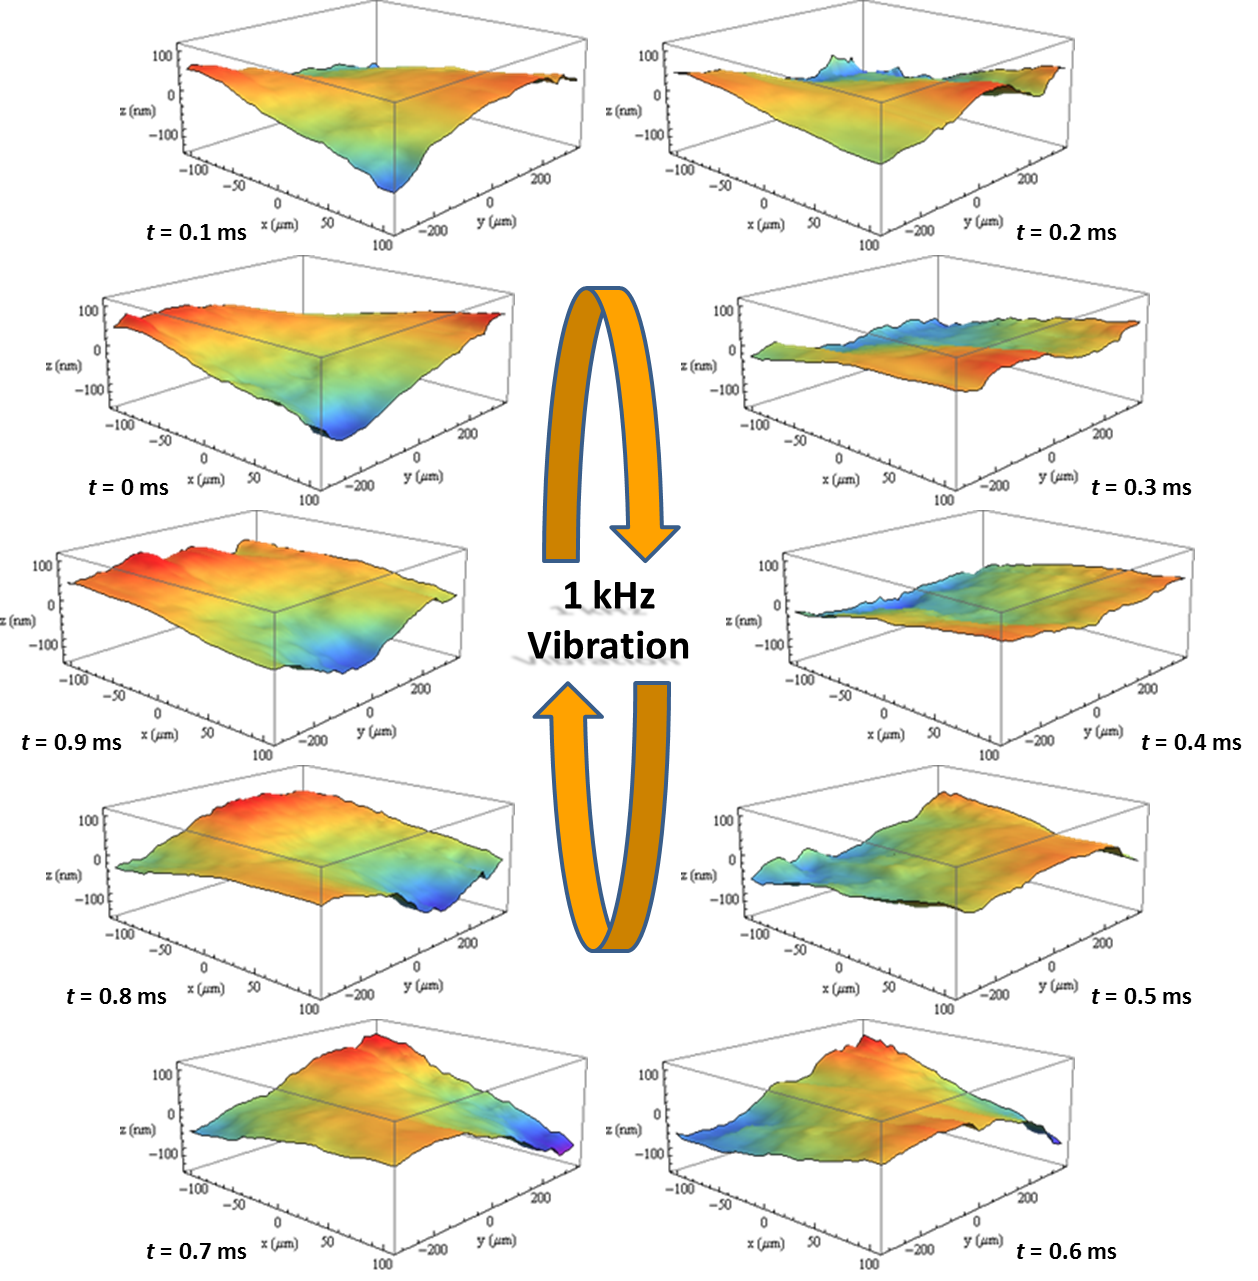
\includegraphics[scale=1]{PW2013/Figure6.png}
\caption{Surface vibration captured by the HDLS. Frames from 3D scans of a vibrating diaphragm by the HDLS show a period of nanomechanical vibrations at 1 kHz. Only one every ten scan is shown here.}
\label{fig:PW2013_Figure6}
\end{figure}

Finally, as an example of the HDLS’ biomedical utility, we demonstrated high-precision high-throughput flow cytometry using the HDLS. Low spatial resolution of conventional flow cytometers causes a considerable number of false positive events that result in statistical error in subpopulation analysis. For instance, they are not effective for detection of multiple cells (i.e., doublets, triplets, etc.) (Figure \ref{fig:PW2013_Figure7}a). We used inertial focusing microfluidic technology28 to precisely align otherwise randomly positioned cells in a single stream with no need for sheath flow (Figure \ref{fig:PW2013_Figure7}b). The microfluidic channel is custom-made on a substrate dielectric mirror from thermoset polyester (TPE) for stability, robustness, and increased precision of cell focusing. HDLS pulses scan the stream of cells, and the forward scattering is reflected back by the substrate mirror for measurement. 

We tested the performance of the HDLS and conventional flow cytometer for size-based identification of white blood cells and MCF7 breast cancer cells (Figure \ref{fig:PW2013_Figure7}c). Since the HDLS flow cytometer is more precise in distinguishing multiple cells e.g. doublets, the count of white blood cells that have unusually larger size is reduced, and therefore, the false positive rate decreases. This improvement in size-based classification of MCF7 breast cancer cells from white blood cells is more evident in comparison of receiver operating characteristic (ROC) curves of the HDLS and conventional flow cytometer (figure 2-7d). We observed that for the same specificity, the sensitivity of our method is significantly higher than that of the conventional flow cytometer. 
 
\begin{figure}[htb!]
\centering
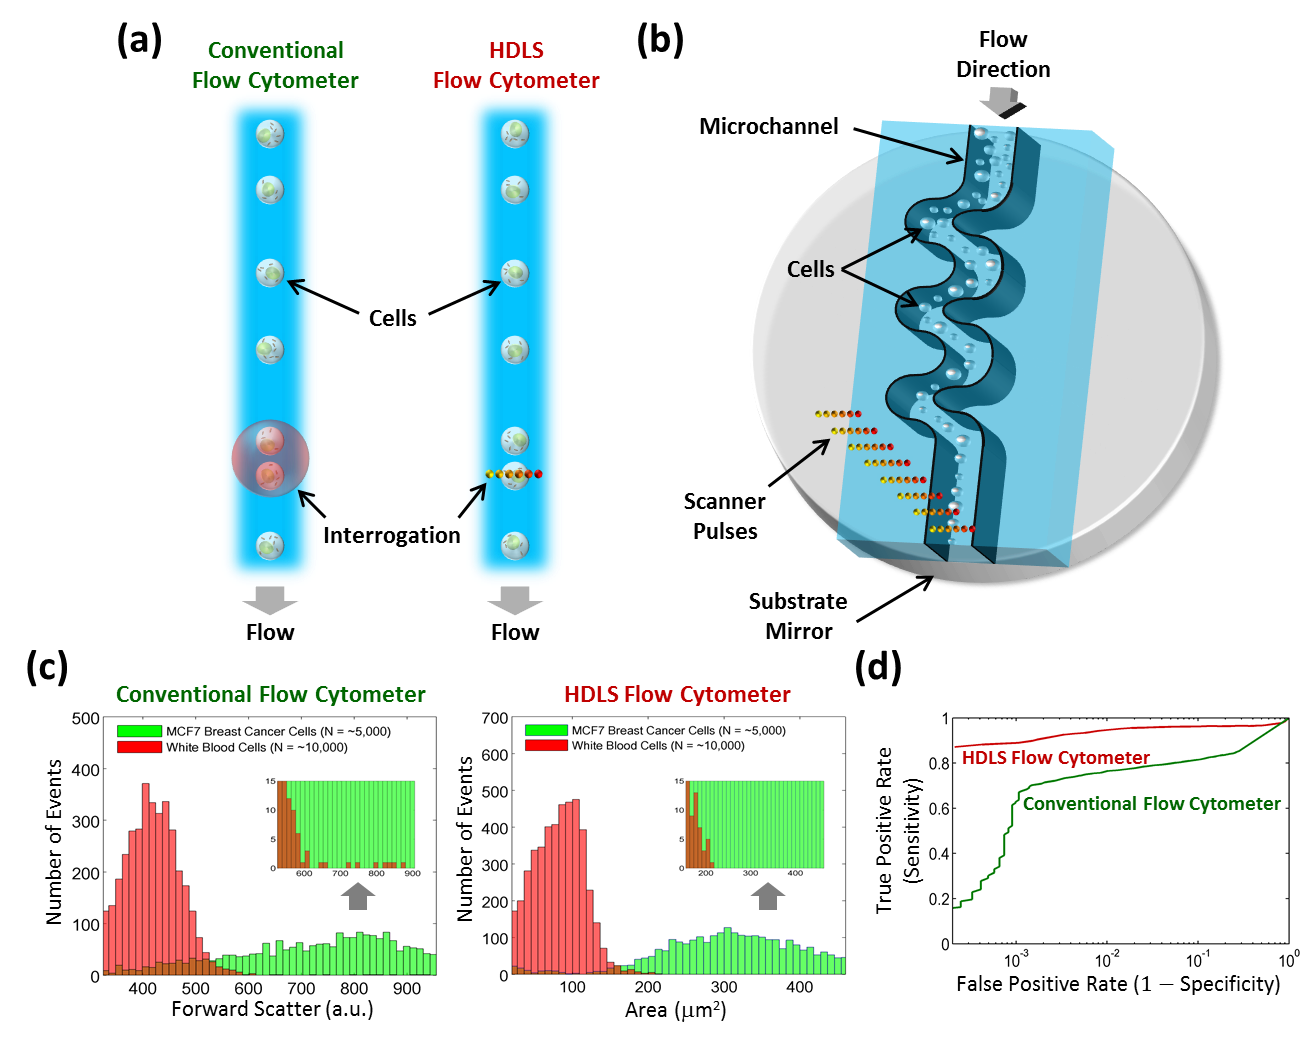
\includegraphics[scale=1]{PW2013/Figure7.png}
\caption{Comparison of conventional and HDLS flow cytometers. (a) In regular flow cytometry, a single interrogation beam covers the desired field of view in the channel. Therefore, it does not efficiently differentiate multiple cells such as doublets. In HDLS flow-cytometer, diffraction limited wavelength components of the interrogation beam cover the required field of view, and extract high-resolution spatial information of the sample. HDLS data can be used to identify abnormalities e.g. multiple cells and result in a lower statistical error. (b) In our demonstration of HDLS flow cytometer, an inertial focusing microfluidic channel with a dielectric mirror substrate is used to order randomly distributed cells into a single stream. The microfluidic device was fabricated using standard replica molding methods in thermoset polyester (TPE) to ensure stability. HDLS scan pulses are focused on the stream. Forward-scattered light from the cells is reflected by substrate mirror and collected by an objective lens. (c) Identical samples of white blood cells and MCF7 breast cancer cells are measured separately with conventional and HDLS flow cytometers. There is a considerable overlap in forward scattering range of these cell types for a conventional flow cytometer. However, this overlap decreases significantly for HDLS flow cytometer measurements because white blood cell multiples are not identified as MCF7 cancer cells. (d) Receiver operating characteristic (ROC) curves based on identification of white blood cells and MCF7 breast cancer cells show that without sacrificing throughput, HDLS flow cytometer achieves higher specificity and sensitivity than a conventional flow cytometer.}
\label{fig:PW2013_Figure7}
\end{figure}

References
1.	marshall2011handbook
2.	fujii2005laser
3.	Ddotson2003fundamentals
4.	popescu2006optical
5.	gobel2006imaging
6.	pawley2010handbook
7.	denk1990two
8.	wandinger2005lidar
9.	schwarz2010mapping
10.	sinha2010vibration
11.	pelesko2002modeling
12.	osten2006optical
13.	horn1986robot
14.	hoffman2006confocal
15.	tarnok2002clinical
16.	vacca2009laser
17.	mahjoubfar2011high
18.	conant2002micromachined
19.	pape1994design
20.	yaqoob2004passive
21.	boudoux2005rapid
22.	goda2012hybrid
23.	kelkar1999time
24.	chou2007femtosecond
25.	goda2009theory
26.	goda2009serial
27.	goda2008amplified
28.	di2009inertial                         % etc.
\chapter{Label-free high-throughput cell screening}

Flow cytometry is a powerful tool for cell counting and biomarker detection in biotechnology and medicine especially with regards to blood analysis. Standard flow cytometers perform cell type classification both by estimating size and granularity of cells using forward- and side-scattered light signals and through the collection of emission spectra of fluorescently-labeled cells. However, cell surface labeling as a means of marking cells is often undesirable as many reagents negatively impact cellular viability or provide activating/inhibitory signals, which can alter the behavior of the desired cellular subtypes for downstream applications or analysis. To eliminate the need for labeling, we introduce a label-free imaging-based flow cytometer that measures size and cell protein concentration simultaneously either as a stand-alone instrument or as an add-on to conventional flow cytometers. Cell protein concentration adds a parameter to cell classification, which improves the specificity and sensitivity of flow cytometers without the requirement of cell labeling. This system uses coherent dispersive Fourier transform to perform phase imaging at flow speeds as high as a few meters per second.

\section{Introduction}

Cell protein content measurement can be used in many biomedical applications such as blood doping detection \cite{grover2011measuring}, infection monitoring \cite{mrema1979concentration}, drug development and screening \cite{chun2012rapidly}, studies of necrosis and apoptosis \cite{martin1990hl,wyllie1982hormone}, cell cycle progression and differentiation \cite{wolff1972separation,maric1998buoyant,bista2011quantification}, and in cancer diagnostics \cite{bosslet1981rapid,phillips2012quantification,phillips2012optical}. Current methods for cell protein concentration measurement include electrical methods based on dielectrophoresis \cite{gupta2012apostream}, mechanical methods based on microchannel cantilevers \cite{grover2011measuring}, and optical methods based on scattering patterns \cite{tycko1985flow}, emission spectra of external cavity lasers \cite{liang2007determining}, and holographic and phase microscopy \cite{rappaz2005measurement,curl2005refractive,lue2009live,gorthi2012phase}. These methods are either inherently too slow for high-speed flow cytometry applications or require feedback mechanisms \cite{popescu2006optical} to provide necessary precision. Furthermore, size-based classification can also be used for label-free identification of cells of interest in a suspension stream \cite{vona2000isolation}. However, due to significant overlap of size ranges between most mammalian cells, size-based technologies require additional layers of parametric gating to be useful as a diagnostic tool \cite{di2013hyperspectral}.  It is known that the refractive index of a cell is proportional to its protein content \cite{barer1954refractometry}. As such, the simultaneous measurement of refractive index and size of cells would be predicted to provide two independent parameters for cell classification.

In this chapter, we propose a fast and high-precision optical cell density and size measurement method based on serial time-encoded amplified microscopy (STEAM) \cite{goda2009serial}. STEAM is a continuous imaging technique that captures tens of million frames-per-second with sub-nanosecond shutter speed. However, earlier versions of STEAM were dependent on cell labeling due to low intensity contrast of individual cells \cite{goda2012high}. Here, we introduce a new configuration of STEAM capable of high-speed phase microscopy and demonstrating label-free single-cell classification and diagnostics. In addition, we demonstrate a new design of STEAM that minimizes loss and chromatic aberration, decreases polarization sensitivity, and results in a smaller footprint \cite{fard2011nomarski}. In contrast to previous implementations of STEAM, which were based on refractive optics, the new design employs reflective optics.

The basic principle of STEAM involves two steps both performed optically. In the first step, the spectrum of a broadband optical pulse is converted by a spatial disperser into a rainbow that illuminates the target. Therefore, the spatial information (image) of the object is encoded into the spectrum of the resultant reflected or transmitted rainbow pulse. A 1D rainbow is used in flow imaging as the flow causes the cell to be scanned in the second dimension. In the second step, the spectrum of the image-encoded pulse is mapped into a serial temporal signal that is stretched in time to slow it down such that it can be digitized in real-time \cite{goda2013dispersive}. This optically-amplified time-stretched serial stream is detected by a single-pixel photodetector and the image is reconstructed in the digital domain. Subsequent pulses capture repetitive frames, hence the laser pulse repetition rate corresponds to the frame rate of STEAM and the shutter speed (exposure time) corresponds to the temporal width of the pulse. The key innovations in STEAM that enable high speed real-time imaging are photonic time stretch for digitizing fast images in real-time and the optical image amplification for compensating the low number of photons collected during the ultra-short shutter time.

The contrast limitations of label-free single-cell imaging of STEAM led us to develop a derivative of STEAM, referred to as Coherent-STEAM, to capture phase images of cells in flow. We use a Michelson interferometer to map the phase image of cells into the spectrum of broadband optical pulses. This phase imaging technique exploits the fast shutter speed of STEAM to freeze path length fluctuations of interferometer arms and attains nanometer phase resolution with no need for feedback stabilization of the interferometer \cite{mahjoubfar2011high,goda2012hybrid,mahjoubfar20133d}. We use Coherent-STEAM to measure the refractive index of individual cells in an imaging flow cytometer by simultaneous measurement of size and total optical phase-shift induced by the cells. As an example, we use our label-free STEAM-based cell classifier to distinguish OT-II T cell hybridoma from SW480 epithelium cancer cells. We show that adding protein concentration to size as an additional classification parameter increases accuracy and specificity in flow cytometry.

\section{Experimental setup}

A mode-locked fiber laser generates pulses at 1565 nm with a repetition rate of 36.128 MHz and a pulse width slightly less than 100 fs (Figure Figure \ref{fig:BOE2013_Figure1}). Pulses are spectrally broadened with a highly nonlinear fiber to approximately 100 nm bandwidth \cite{boyraz2000broadband}. A short dispersion compensating fiber with an overall dispersion of 60 ps/nm is used to temporally broaden pulses to 1.2 ns, so an erbium doped fiber amplifier (EDFA) can amplify them without any distortion. Amplified pulses enter a coarse wavelength division multiplexing (WDM) filter, and the output of 1591 nm channel is used to shape laser pulses with a considerably flat spectrum over 1581 nm to 1601 nm bandwidth. These pulses pass through an optical circulator and are coupled to free-space with a fiber collimator.

\begin{figure}[htb!]
\centering
\includegraphics[scale=1]{BOE2013/Figure1.png}
\caption{Optical setup of Coherent-STEAM. A Coherent-STEAM setup is formed by combination of STEAM and a Michelson interferometer. A pair of diffraction gratings generates a 1D rainbow with different wavelength components imaging different points on the cells flowing in a microfluidic channel. A pellicle beam-splitter and two identical long working-distance objective lenses are used to form the interferometer for phase measurement. Back apertures of objective lenses are fully illuminated with each wavelength component of the broadband mode-locked laser pulses to ensure diffraction-limited resolution. An amplified time-stretch system chirps, stretches, and amplifies each pulse, so that different wavelength components reach the photodetector serially. A very shallow microfluidic channel with hydrodynamic focusing is designed and fabricated to align cells within the focal depth of the system.}
\label{fig:BOE2013_Figure1}
\end{figure}

Free-space laser pulses are linearly polarized with quarter- and half-wave plates, and then they are spatially dispersed with a pair of reflection diffraction gratings, so that each wavelength component of the collimated beam is positioned at a different lateral point similar to a rainbow. A pair of 90 degree off-axis parabolic gold-coated mirrors with 152.4 mm and 25.4 mm reflected focal lengths are used to form a beam reducer that shrinks the rainbow beam 6 times. Parabolic gold-coated mirrors are used to minimize loss, aberration, and polarization sensitivity. In addition, a 15 degree off-axis parabolic gold-coated mirror with 635 mm reflected focal length and a 0.4 numerical aperture long working-distance objective lens further shrink the rainbow to about 130 μm field of view. Using reflective optics, we managed to improve the signal-to-noise ratio by about 9 dB. A beam splitter is used to form two arms of a Michelson interferometer. Different wavelength components of the rainbow are focused on a mirror in the reference arm and on the reflective substrate of a microfluidic device in the sample arm. Cells hydrodynamically focused at the center of the channel flow at a velocity of 1.3 m/s. The rainbow pulses pass through the cells and are reflected back by the mirror substrate of the microfluidic device. The total bandwidth of the pulses interrogating the cells in our Coherent STEAM is less than 20 nm centered at 1590 nm, giving a negligible fractional bandwidth of 1.3\%. Therefore, the color-dependency of absorption is very small and can be easily neglected. The reflected pulses from the microfluidic device and reference mirror interfere at the beam splitter and return to the fiber, where they are directed with the optical circulator to an amplified time-stretch system.

The amplified time-stretch system is a combination of a Raman amplifier and a dispersive fiber to perform dispersive Fourier transform \cite{goda2013dispersive}. Four Raman pump lasers at 1450 nm, 1470 nm, 1490 nm, and 1505 nm are used to amplify the signal for about 15 dB over the whole optical bandwidth uniformly. The dispersive fiber chirps and stretches each pulse in time to about 27 ns. So, different wavelength components reach the photodetector serially. An analog-to-digital convertor (ADC) with a sampling rate of 50 GSps and 20 GHz bandwidth is used to acquire the output signal of the photodetector.

The photodetector output signal, $I(t)$, is digitized and recorded by the ADC (Figure \ref{fig:BOE2013_Figure2}a). This signal shows sequential laser pulses. Each pulse is used to form one line image. Therefore, the boundaries of pulses are determined precisely, and each pulse is saved separately as a frame for further processing (Figure \ref{fig:BOE2013_Figure2}b). The analytic form of each pulse is generated using Hilbert transformation after the low frequency components corresponding to intensity variations are filtered out \cite{ikeda2005hilbert}. The phase component of this analytic form is extracted, while its amplitude component is discarded (Figure \ref{fig:BOE2013_Figure2}c). Because the phase varies over a wide range (much larger than $2 \pi$ radians), it shows unrealistic discontinuities. An unwrapping algorithm is used to fix these discontinuities, and the result shows an approximately linear phase increase over the time for each pulse or frame (Figure \ref{fig:BOE2013_Figure2}d). The unwrapping algorithm adds multiples of $\pm 2 \pi$ to make the absolute jumps between consecutive samples in a frame smaller than $\pi$ radians when they are greater than $\pi$ radians. If the linear component of the phase, which corresponds to the fringe (modulation) frequency, $f_m$, due to the interferometer arms’ length mismatch, and the background phase level, $\varphi_0$, are subtracted, the phase shift induced by the cells in the optical pulse can be observed (Figure \ref{fig:BOE2013_Figure2}e); i.e. 
\begin{equation}
\Delta\varphi(t)= unwrap(\arg(I_{BP}(t)+j \cdot \hat{I}_{BP}(t))) - 2 \pi f_m t - \varphi_0
\end{equation}
in which $I_{BP}(t)$ is a band-pass filtered form of $I(t)$ with only spectral features modulated at $f_m$, and $\hat{I}_{BP}(t)$ is the Hilbert transform of $I_{BP}(t)$. Many phase line images generated from subsequent frames are combined to form a spatial map of optical path difference (OPD) in two dimensions (Figure \ref{fig:BOE2013_Figure2}f). Since we know the mapping of space to time from the rainbow characteristics and flow speed, OPD at each point is calculated as
\begin{equation}
OPD(x,y) = \frac{\lambda(x)}{2 \pi} \Delta\varphi(x,y)
\end{equation}
where $x$ and $y$ are coordinates in the rainbow and flow directions, respectively; $\lambda(x)$ is the wavelength at position $x$ along the rainbow; and $\Delta\varphi(x,y)$ is the phase shift induced by the cell at point $(x,y)$.

\begin{figure}[htb!]
\centering
\includegraphics[scale=1]{BOE2013/Figure2.png}
\caption{Digital signal processing of Coherent-STEAM. (a) The photodetector output signal is digitized and recorded by an ADC. This signal shows sequential laser pulses. (b) Each pulse is saved separately as a frame for further processing. (c) The analytic form of high-frequency components of each pulse is generated using Hilbert transformation, and the phase component of this analytic form is extracted. (d) An unwrapping algorithm is used to fix unrealistic phase jumps, and the result shows an approximately linear phase increase. (e) If the phase component of the interferometer fringe frequency is removed, the phase induced by cells in optical pulse can be seen. (f) Many of these line images generated from subsequent frames are used to form a spatial map of optical path difference in two dimensions, which is used for cell characterization.}
\label{fig:BOE2013_Figure2}
\end{figure}

Spatial map of optical path difference can be used to extract the refractive index contrast between the cell and the surrounding liquid.  If the thickness of the cell at point $(x,y)$ is $t(x,y)$,
\begin{equation}
OPD(x,y) = 2 \Delta n_{cell} \cdot t(x,y)
\label{eqn:BOE2013_Equation3}
\end{equation}
where $\Delta n_{cell} = n_{cell} - n_{liquid}$ in which $n_{cell}$ and $n_{liquid}$ are the refractive indices of the cell and the surrounding liquid, respectively. The factor 2 is to account for the fact that each wavelength component passes the cell twice in Michelson interferometer. If we integrate Equation \eqref{eqn:BOE2013_Equation3} over the area of the cell, we can derive an average refractive index contrast, which corresponds to protein concentration of the cell:
\begin{equation}
\Delta n_{cell} = \frac{\iint_{cell} OPD(x,y) \ud x \ud y}{2V_{cell}}
\label{eqn:BOE2013_Equation4}
\end{equation}
where $V_{cell} = \iint_{cell} t(x,y) \ud x \ud y$ is the volume of the cell. Most of the cells relax to a spherical shape when they are released from substrates and brought into suspension \cite{revel1974adhesion,whur1977substrate}. Therefore, if we know the diameter of the cell, $d_{cell}$, we can estimate its volume as $V_{cell} \approx \pi d_{cell}^3/6$.

\section{Results and discussion}
Spherical polystyrene beads with a NIST traceable diameter of 5 μm are used to calibrate the image processing algorithm for size measurements. A custom designed algorithm in CellProfiler software \cite{carpenter2006cellprofiler} is used to detect the beads or cells in spatial map of optical path difference (Figure \ref{fig:BOE2013_Figure3}). Bead or cell diameter is measured along the rainbow direction to eliminate size measurement inaccuracies caused by fluctuations of flow speed (Figure \ref{fig:BOE2013_Figure3}a). Due to limited optical resolution of the setup, the bead or cell edges are blurred, generating a small phase signal outside of the diameter bars. The diameter along the rainbow direction is equal to the diameter along the interrogation optical beam for spherical-shape beads or cells in suspension, including the samples in our experiments. 

\begin{figure}[htb!]
\centering
\includegraphics[scale=1]{BOE2013/Figure3.png}
\caption{Calibration with NIST traceable beads. Polystyrene beads with a NIST traceable diameter of 5 μm are used to calibrate the image processing algorithm for size measurements. (a) A custom designed image processing algorithm in CellProfiler software is used to find the beads in spatial map of optical path difference and measure the diameter. (b) Histogram of bead diameters demonstrates the measured size distribution has an expected mean of 5 µm and a standard deviation within the range of optical resolution limit. (c) Since all the beads are made out of the same material, the coefficient of variation for refractive indices ($0.014/1.57 = 0.89\%$) is much smaller than that of diameters ($0.405/5.06 = 8.00\%$).}
\label{fig:BOE2013_Figure3}
\end{figure}

Histogram analysis of bead diameter distribution for more than one hundred beads with corresponding Gaussian fit to measurements demonstrates that the measured size distribution has a standard deviation of 0.4 μm and an expected mean of 5 μm (Figure \ref{fig:BOE2013_Figure3}b). The broadening in the distribution is caused by the limited lateral optical resolution of the Coherent-STEAM setup. This resolution is measured by the knife-edge method and is about 2.5 μm. Therefore, the standard deviation of the bead size distribution is well below the optical resolution.

We also measured the refractive index contrast of each bead and the surrounding liquid using Coherent-STEAM. Assuming that the refractive index of water is 1.317 at the 1581 nm to 1601 nm bandwidth, we derived the refractive index of the beads using Equation \eqref{eqn:BOE2013_Equation4}. Analysis of the bead refractive indices and corresponding Gaussian fit demonstrates that the beads have a mean refractive index of 1.57 with a standard deviation of 0.014 (Figure \ref{fig:BOE2013_Figure3}c). We observe that the coefficient of variation for the bead refractive indices is 0.89\%, which is much smaller than the coefficient of variation for the bead diameters (8.00\%). This is expected because all the beads are made out of the same material, while their diameter measurements are effected by dispersity of the size and limited spatial resolution of the setup.

We used the calibrated Coherent-STEAM setup to measure cell diameter and refractive index contrast (as a measure for protein concentration) simultaneously. Different types of cells have different mean diameters and protein concentrations; however, both of these parameters have a broad range of variations for each cell type. We see that identification of cells is more specific using both of these parameters simultaneously, instead of each individually. Images of OTII (Figure \ref{fig:BOE2013_Figure4}a) and SW480 (Figure \ref{fig:BOE2013_Figure4}b) cells taken by Coherent STEAM setup demonstrate that the cells are spherical in the microfluidic channel. In Figure \ref{fig:BOE2013_Figure4}c, scattering plot of cell protein concentration (refractive index difference) versus diameter is shown for these cells. Using points in a normal range of protein concentration and sliding the detection limit along the depicted direction (perpendicular to the optimum classification line), a receiver operating characteristic (ROC) curve is generated (Figure \ref{fig:BOE2013_Figure4}d). Comparing the ROC curve of individual parameters (e.g. size measurement only) to that of simultaneous measurement, it becomes obvious that the detection sensitivity has improved considerably. 

\begin{figure}[htb!]
\centering
\includegraphics[scale=0.65]{BOE2013/Figure4.png}
\caption{Cell classification based on size and protein concentration measurement by Coherent-STEAM; Images of (a) SW480 and (b) OTII cells taken by Coherent STEAM setup show that they are spherical. (c) Scattering plot of cell protein concentration versus diameter is shown for OTII (blue) and SW480 (green) cells. (d) Comparison of the ROC curves of size measurement only (purple line) to that of simultaneous size and protein concentration measurement (orange line) shows significant improvement in sensitivity.}
\label{fig:BOE2013_Figure4}
\end{figure}

\section{Conclusion}

In summary, we demonstrated a new type of imaging flow cytometry based on coherent stretched-time-encoded amplified microscopy, which is capable of classifying cells in flow rates as a high as a few meters per second. Coherent-STEAM measures size and total optical path difference of cells simultaneously and extracts the refractive index, which corresponds to the protein concentration of the cells, as an additional parameter for classification. As illustrated in our experimental results, separation of two cell types was significantly enhanced by adopting the additional protein concentration parameter generated by Coherent-STEAM. We will continue our work with real-time signal processing and cell identification on field-programmable gate arrays (FPGAs) for classification of more than two cell types.

\chapter{Optically amplified detection for biomedical sensing and imaging}

Optical sensing and imaging methods for biomedical applications such as spectroscopy and laser-scanning fluorescence microscopy are incapable of performing sensitive detection at high scan rates due to the fundamental trade-off between sensitivity and speed. This is because fewer photons are detected during short integration times and hence the signal falls below the detector noise. Optical postamplification can, however, overcome this challenge by amplifying the collected optical signal after collection and before photodetection. Here we present a theoretical analysis of the sensitivity of high-speed biomedical sensing and imaging systems enhanced by optical postamplifiers. As a case study, we focus on Raman amplifiers because they produce gain at any wavelength within the gain medium’s transparency window and are hence suitable for biomedical applications. Our analytical model shows that when limited by detector noise, such optically postamplified systems can achieve a sensitivity improvement of up to 20 dB in the visible to near-infrared spectral range without sacrificing speed. This analysis is expected to be valuable for design of fast real-time biomedical sensing and imaging systems.

\section{Introduction} \label{sec:JOSAA2013_Section1}

Fast real-time optical sensing and imaging are essential tools for studying fast transient processes in biomedical applications such as neuroscience \cite{ohki2005functional,golshani2009internally}, laser surgery \cite{slade2000complete}, and extracorporeal shockwaves \cite{delius2002twenty,riehle1987principles}. They are equally important for microfluidic biotechnology applications (e.g., flow cytometry) \cite{goda2009serial,squires2005microfluidics,watson2004introduction} that require high-throughput analysis of a large population of cells and pathogens with minimum error. Another important application is Raman spectroscopy in which high-speed sensing capability is needed to investigate fast chemical changes such as those that occur during combustion \cite{hult2007high} and chemical reactions between biological molecules \cite{epstein1998introduction,petty2006spatiotemporal,siesler2008near}. Some examples of applications that require both high scan rates and high detection sensitivity are laser-scanning confocal microscopy, fluorescence microscopy, coherent anti-Stokes Raman spectroscopy, and two-photon microscopy used to observe neural activity in real time \cite{diaspro2001confocal}. Here even higher throughput is desirable to monitor the dynamics of a large number of neurons simultaneously.
The central requirement for these studies is a signal integration time that is much shorter than the time scale of dynamic processes. This requirement must be satisfied, but is difficult to meet due to the fundamental trade-off between sensitivity (minimum detectable power) and speed; at high scan rates, fewer photons are detected during the short integration time within each scan period. This leads to the loss of sensitivity in high-speed detection as it is limited by detector noise (typically thermal noise in the photodetector).

The reduced sensitivity can be compensated for by the use of high-intensity illumination, which, in fact, is frequently used in industrial applications. However, this approach is not suitable for biomedical applications as it can damage the biological sample. The problem becomes much more severe in microscopy because focusing the light onto the sample with an objective lens results in an extremely high intensity. Another technique used to reduce detector thermal noise is detector cooling. However, this is undesirable as it requires a refrigeration unit to accompany the detector and hence adds significant cost and complexity to the detector design and reduces reliability.

Optical postamplification (after signal collection and before photon-to-electron conversion) can circumvent this fundamental challenge when the detection sensitivity is limited by detector noise (typically thermal noise) \cite{goda2009serial,goda2008amplified,mahjoubfar2011,goda2009theory,tsia2010performance,qian2009real,han2003photonic,goda2013dispersive}. It eliminates the need for high-intensity illumination and cooling and represents a novel method for detecting weak optical signals in biomedical sensing and imaging applications. As shown in Figure \ref{fig:JOSAA2013_Figure1}, an optical postamplifier before the photodetector increases the optical signal while the detector thermal noise is intact and hence improves the sensitivity of the detection system in the thermal noise limited region, which is the case in high-speed sensing and imaging. Unlike detector cooling, optical postamplification can be easily employed before photodetection to improve the sensitivity with no need for modifications of the detector design. 

\begin{figure}[htb!]
\centering
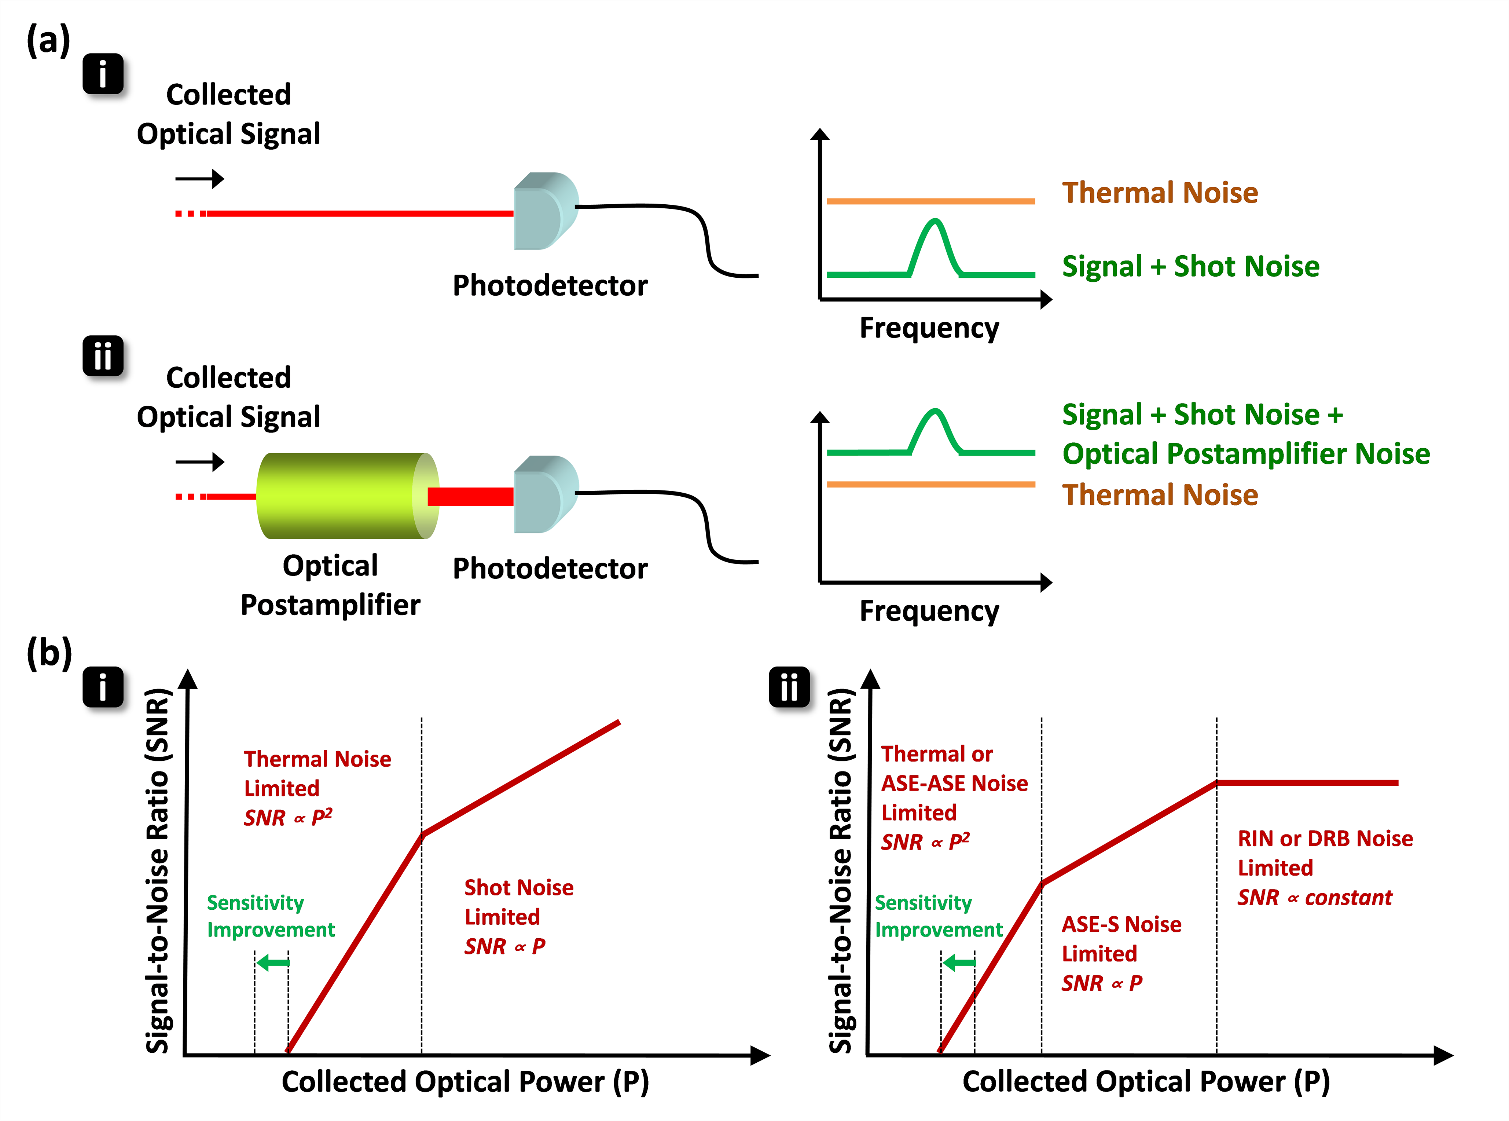
\includegraphics[scale=0.85]{JOSAA2013/Figure1.png}
\caption{Detector sensitivity improvement by an optical postamplifier in high-speed detection. (a) (i) The optical signal is buried in the thermal noise of the photodetector (ii) whereas an optical postamplifier increases the optical signal with the thermal noise intact resulting in an improvement in the sensitivity of the detection system. (b) Comparison of the signal-to-noise ratios for photodetection (i) with and (ii) without an optical postamplifier shows that the optical postamplifier is useful when the detection sensitivity is thermal noise limited because the signal-to-noise ratio is directly proportional to the square of the collected optical power. Here, the signal-to-noise ratio and the collected optical power are both in logarithmic scale. ASE-ASE: amplified spontaneous emission self-beat; ASE-S: amplified spontaneous emission – signal beat; RIN: relative intensity noise; DRB: double Rayleigh backscattering. (These noise components are detailed in Section \ref{sec:JOSAA2013_Section3}.).}
\label{fig:JOSAA2013_Figure1}
\end{figure}

Optical postamplification is fundamentally different from the use of electronic signal intensifiers [e.g. micro-channel plates used in photomultiplier tubes (PMTs) or intensified charge-coupled device (ICCDs)] in that amplification occurs in the optical domain whereas in electronic signal intensifiers, it occurs in the electronic domain. Electronic signal intensifiers are complex vacuum tube devices that require high voltage sources. Also, their scan rates are limited by the fundamental trade-off between gain and bandwidth in all electronic systems \cite{horowitz1989art}. While PMTs are extremely sensitive detectors useful for capturing faint light or even counting single photons, they are unsuitable for continuous high-speed detection due to the limited bandwidth and the dead time caused by their gated operation.

Among different approaches to optical amplification, stimulated Raman scattering (SRS) \cite{agrawal2007nonlinear,islam2002raman} provides several advantages over other methods such as rare-earth doped fiber amplifiers and semiconductor optical amplifiers (SOAs). First, gain is possible at any wavelength as long as a pump is available at a frequency blue-shifted from the signal by the optical-phonon vibrational frequency \cite{agrawal2007nonlinear}. Second, a broad and flexible gain spectrum can be obtained by using multiple pump fields \cite{islam2002raman}. Finally, Raman amplifiers have a lower noise figure than rare-earth doped fiber amplifiers and SOAs \cite{islam2002raman,goda2009demonstration}. For these reasons, Raman amplifiers are routinely employed in fiber-optic communication \cite{islam2002raman}.

Recently, we have reported Raman amplification of a weak optical signal in a single-mode fiber in the 800 nm spectral range for the first time \cite{goda2009demonstration,mahjoubfar2010raman}. This proof-of-principle demonstration has shown potential utility of Raman amplifiers to biomedical sensing and imaging applications. While noise sources associated with Raman amplifiers have been extensively studied in the fiber-optic communication band (1300 - 1600 nm), virtually no such work has been done in the optical spectrum outside of the fiber-optic communication band. However, the short wavelength band (500 - 900 nm) is important for biomedical applications as most of them are conducted in this band in favor of low water absorption and high spatial resolution in imaging.

In this chapter, we theoretically analyze the sensitivity of a detection system enhanced by a Raman fiber amplifier as an optical postamplifier at such short wavelengths. This postamplifier can be easily used in fiber-based biomedical imaging and sensing devices such as fiber-coupled confocal and fluorescence scanning microscopes \cite{bird2002compact,kimura1991confocal}, serial time-encoded microscopes \cite{goda2009serial,tsia2010performance,goda2012hybrid,mahjoubfar2013label}, and fiber-optic biosensors \cite{wolfbeis2004fiber,song2006refractive,piliarik2003surface}. However, it is impractical to employ this fiber amplifier before a free-space imaging or sensing system e.g. a charge-coupled device (CCD) or a complementary metal–oxide–semiconductor (CMOS) image sensor because the fiber coupling losses mostly defeat the benefits of the postamplification. First, we review the basic concept of the Raman amplifier in Section \ref{sec:JOSAA2013_Section2}. We then derive the variances of noise photocurrents associated with the Raman amplifier as well as photodetection in Section \ref{sec:JOSAA2013_Section3}. With the results in Section \ref{sec:JOSAA2013_Section3}, we evaluate and compare the noise current variances and then study the sensitivity of the detection system enhanced by the amplifier in Section \ref{sec:JOSAA2013_Section4}. We also perform numerical simulations to obtain a set of parameter values that optimize the performance of the detection system at various wavelengths. In Section \ref{sec:JOSAA2013_Section5}, we conclude this chapter.

\section{Raman amplification as an optical postamplifier} \label{sec:JOSAA2013_Section2}

Raman amplification is an optical process based on the phenomenon of SRS \cite{agrawal2007nonlinear,islam2002raman}. As shown in Figure \ref{fig:JOSAA2013_Figure2}, in SRS an input field (called the Stokes field) stimulates the inelastic scattering of a blue-shifted pump field inside an optical medium mediated by its vibrational modes (called optical phonons). As with the rare-earth doped fiber amplifiers, Raman amplifiers based on the process of Raman amplification are often used to increase optical signals in fiber-optic communications with transmission fibers as gain media \cite{agrawal2007nonlinear,islam2002raman}.

A typical Raman amplifier is schematically shown in Figure \ref{fig:JOSAA2013_Figure2}. It consists of a single-mode silica fiber as a gain medium, an input weak field (Stokes field), and one or two continuous-wave pump fields that couple into and out of the fiber via duplexers such as fiber-based wavelength-division multiplexers or dichroic beamsplitters in free space. In many cases, the fiber is bidirectionally pumped in the forward and backward directions to optimize the performance of the amplifier.

\begin{figure}[htb!]
\centering
\includegraphics[scale=1]{JOSAA2013/Figure2.png}
\caption{Energy diagram of stimulated Raman scattering (SRS) and basic schematic of a SRS-based optical postamplifier. (a) Raman amplification is an optical process based on the phenomenon of SRS in which the input field (called the Stokes field) stimulates the inelastic scattering of a blue-shifted pump field inside an optical medium mediated by its vibrational modes (optical phonons). (b) A typical Raman amplifier consists of a single-mode silica fiber (gain medium), an input at the Stokes frequency, and one or two pump fields that couple into and out of the fiber via duplexers such as wavelength-division multiplexers or dichroic beamsplitters. The fiber is bidirectionally pumped in the forward and backward directions to optimize the performance of the amplifier.}
\label{fig:JOSAA2013_Figure2}
\end{figure}

Raman amplification in an optical fiber is governed by the following coupled equations:
\begin{eqnarray}
\frac{\ud I_s}{\ud z} &=& g_R I_p I_s - \alpha_s I_s,\label{eqn:JOSAA_Equation_1}\\
\frac{\ud I_p}{\ud z} &=& -\frac{\omega_p}{\omega_s} g_R I_p I_s- \alpha_p I_p,\label{eqn:JOSAA_Equation_2}
\end{eqnarray}
where $I_s$ and $I_p$ are the intensities of the Stokes and pump fields, respectively, $\omega_s$ and $\omega_p$ are the optical frequencies of the Stokes and pump fields, respectively, $\alpha_s$ and $\alpha_p$ are the loss coefficients of the fiber at the Stokes and pump frequencies, respectively, $g_R$ is the Raman gain coefficient, and $z$ is the propagation distance.

Assuming that the pump field is much more powerful than the input signal (which is often the case) and hence undepleted, the first term on the right hand side in Equation \eqref{eqn:JOSAA_Equation_2} can be ignored and the pump intensity decreases exponentially in the fiber. If the fiber is bidirectionally pumped, the total pump intensity at an arbitrary position in the fiber can be obtained from Equation \eqref{eqn:JOSAA_Equation_2} and is given by
\begin{equation}
I_p(z) = I_p^f(z) + I_p^b(z),\label{eqn:JOSAA_Equation_3}
\end{equation}
where 
\begin{eqnarray}
I_p^f(z) &=& I_p^f(0) \mathrm{e}^{-\alpha_p z},\label{eqn:JOSAA_Equation_4a}\\
I_p^b(z) &=& I_p^b(L) \mathrm{e}^{-\alpha_p (L-z)}.\label{eqn:JOSAA_Equation_4b}
\end{eqnarray}
Here $L$ is the total length of the fiber, $I_p^f(0)$ and $I_p^b(L)$ are the intensities of the forward and backward pump fields at fiber ends, respectively, which can be obtained from the pump powers in the forward and backward directions,
\begin{eqnarray}
I_p^f(0) &=& \frac{P_p^f(0)}{\pi(d_p/2)^2},\label{eqn:JOSAA_Equation_5a}\\
I_p^b(L) &=& \frac{P_p^b(L)}{\pi(d_p/2)^2},\label{eqn:JOSAA_Equation_5b}
\end{eqnarray}
where $P_p^f(0)$ and $P_p^b(L)$ are the forward and backward pump powers, respectively, and $d_p$ is the mode field diameter of the pump fields in the fiber. Likewise, the Stokes intensity can also be obtained from the input power (Stokes power),
\begin{equation}
I_s(z) = \frac{P_s(z)}{\pi(d_s/2)^2},\label{eqn:JOSAA_Equation_6}
\end{equation}
where $d_s$ is the mode field diameter of the Stokes field in the fiber. Here we have assumed that the forward and backward pump fields are uncorrelated and do not interfere with each other in the fiber.
Substituting Equation \eqref{eqn:JOSAA_Equation_3} into Equation \eqref{eqn:JOSAA_Equation_1}, the intensity of the Stokes field at an arbitrary point in the fiber, $I_s(z)$, can be obtained, and hence, the net gain is also found to be
\begin{equation}
G(z)=\frac{I_s(z)}{I_s(0)}=\exp\left\{\frac{g_R}{\alpha_p} \left[I_{p}^f(0)\left(1-\mathrm{e}^{-\alpha_p z}\right)+I_{p}^b(L)\left(\mathrm{e}^{-\alpha_p (L-z)}-\mathrm{e}^{-\alpha_p L}\right)\right]- \alpha_s z\right\},\label{eqn:JOSAA_Equation_7}
\end{equation}
where $I_s(0)$ is the intensity of the input Stokes field before entering the fiber.

\section{Limiting noise sources} \label{sec:JOSAA2013_Section3}

In order to evaluate the performance of the Raman amplifier, or more specifically, to study the sensitivity of a detection system enhanced by the amplifier, it is important to understand limiting noise sources associated with the amplifier. In this section, we derive analytical forms for such noise components. We then evaluate and compare them using realistic parameter values in the next section.

\subsection{Double Rayleigh backscattering noise}

Rayleigh scattering is the elastic scattering of light by particles (i.e., atoms and molecules) with dimensions which are much smaller than the wavelength of the light. Rayleigh scattering by molecules in the fiber medium (typically glass) is a fundamental loss mechanism in all optical fibers. While most of the scattered light escapes through the cladding, a small portion of the light can stay in the fiber core and propagate backward in the fiber. This backward-propagating scattered light is normally very weak, but it can be amplified by distributed Raman amplification in the fiber. The amplified backward-propagating scattered light can again be scattered and propagate along with the signal in the forward direction. This causes a delayed crosstalk in-band noise that is amplified by the process of SRS in the fiber \cite{agrawal1997fiber,kim2002reflection}. It is called double Rayleigh backscattering (DRB) noise \cite{islam2004raman,lewis2000characterization} and is known to play a critical role in limiting the performance of Raman amplifiers in long-haul fiber-optic communication systems \cite{hansen1998rayleigh}.

The crosstalk-to-signal ratio or fraction of the signal power that is scattered by DRB and amplified is given by \cite{nissov1999rayleigh}
\begin{equation}
f_{DRB} = r_s^2 \int_0^L G^{-2}(z) \int_z^L{G^2(z') \ud z'} \ud z,\label{eqn:JOSAA_Equation_8}
\end{equation}
where $r_s$ is the Rayleigh baskscattering coefficient. Since this is proportional to the Rayleigh scattering loss, it is inversely proportional to $\lambda_s^4$, where $\lambda_s$ is the wavelength of the input (Stokes) field. Therefore, the DRB noise is an important limiting noise factor at shorter (visible) wavelengths used in biomedical applications than in the fiber-optic communication links because they operate in the longer-wavelength infrared band.

The variance of the DRB noise photocurrent produced by the photodiode is given by \cite{headley2005raman}
\begin{equation}
\left\langle \delta i_{DRB}^2\right\rangle = 2 f_{DRB} [r_d G(L) P_s(0)]^2,\label{eqn:JOSAA_Equation_9}
\end{equation}
where $r_d$ is the responsivity of the photodetector, and $P_s(0)$ is the input Stokes power. The factor of 2 in the equation accounts for the two polarization modes of the fiber.

\subsection{Pump-to-Stokes relative intensity noise transfer}

Every laser including pump lasers in Raman amplifiers has intensity fluctuations called relative intensity noise (RIN) which typically originate from laser cavity vibration, instability in the laser gain medium (caused by the feedback between electron and photon populations), or transferred intensity noise from a pump source. As the Raman amplifier is powered by one or more pump fields, their RIN can transfer to the amplified (Stokes) signal through the process of SRS.

Using the RIN calculation technique described for a singly-pumped Raman amplifier in Ref. \cite{fludger2001pump}, the transfer function of the pump RIN to the Stokes RIN in bidirectionally pumped Raman amplifiers is found to be
\begin{eqnarray}
&&\hspace{-0.7cm}RIN_s(f) = \nonumber\\
&&\hspace{-0.5cm}\left\{\frac{v_s\left[\alpha_s L + \ln G(L)\right]}{L_{eff}}\right\}^2  
 \left\{RIN_p^f(f) \left[\frac{P_p^f(0)}{P_p^f(0)+P_p^b(L)}\right]^2 \left[\frac{1-2\mathrm{e}^{-\alpha_p L}\cos(bfL/v_s)+\mathrm{e}^{-2 \alpha_p L}}{(\alpha_p v_s)^2+(b f)^2}\right] \right.\nonumber\\
&&\hspace{-0.5cm} \left.+RIN_p^b(f) \left[\frac{P_p^b(L)}{P_p^f(0)+P_p^b(L)}\right]^2 \left[\frac{1-2\mathrm{e}^{-\alpha_p L}\cos(4 \pi f L/v_s)+\mathrm{e}^{-2 \alpha_p L}}{(\alpha_p v_s)^2+(4 \pi f)^2}\right]\right\},\label{eqn:JOSAA_Equation_10}
\end{eqnarray}
where $f$ is the electrical frequency of the detection circuitry (also called the sideband frequency of the optical carrier), $RIN_p^f(f)$ and $RIN_p^b(f)$ are the RIN coefficient of the forward and backward pump lasers, respectively, $v_s$ is the group velocity of the Stokes field, $L_{eff}$ is the effective length of the fiber at the pump wavelength and is given by
\begin{equation}
L_{eff}=\frac{1-\exp(-\alpha_p L)}{\alpha_p},\label{eqn:JOSAA_Equation_11}
\end{equation}
and a constant, $b$, is defined in terms of the difference in group velocity between the pump and Stokes fields by
\begin{equation}
b = 2\pi\left(1-\frac{v_s}{v_p}\right).\label{eqn:JOSAA_Equation_12}
\end{equation}
Here $v_p$ is the group velocity of the pump fields. The first and second terms in Equation \eqref{eqn:JOSAA_Equation_10} account for the RIN transfer from the forward and backward pump RINs to the Stokes RIN, respectively.

The variance of the RIN transfer noise photocurrent produced by the photodiode is found by integrating the beat between the Stokes field and the pump-RIN-transferred Stokes noise over the electrical bandwidth of the photodetector, $B_e$, to be
\begin{equation}
\left\langle \delta i_{RIN}^2\right\rangle = \int_0^{B_e}RIN_s(f) [r_d G(L) P_s(0)]^2 \ud f.\label{eqn:JOSAA_Equation_13}
\end{equation}

\subsection{Amplified spontaneous emission noise}

When an optical gain medium is pumped to produce population inversion (hence gain), the random spontaneously emitted light is amplified by the process of stimulated emission. This process is called amplified spontaneous emission (ASE) and produces photons that have random phases relative to the signal and appear as noise. The SRS-induced ASE noise gives rise to two beat-noise signals that appear at baseband frequencies: (1) beating of the Stokes field with the ASE and (2) beating of the ASE with itself. The variances of these noise photocurrents generated at the photodiode are given by \cite{headley2005raman,agrawal2001applications}
\begin{eqnarray}
\left\langle \delta i_{s-ASE}^2\right\rangle &=& 4 r_d^2 G(L) P_s(0) S_{ASE} B_e, \label{eqn:JOSAA_Equation_14}\\
\left\langle \delta i_{ASE-ASE}^2\right\rangle &=& 4 r_d^2 S_{ASE}^2 B_e \left(B_o-\frac{B_e}{2}\right), \label{eqn:JOSAA_Equation_15}
\end{eqnarray}
where $B_o$ is the optical bandwidth of the photodetector, $B_e$ is the electrical bandwidth of the detection system ($B_e$ is assumed to be $< B_o/2$), and $S_{ASE}$ is the spectral density of the ASE defined by \cite{kogelnik1964considerations}
\begin{equation}
S_{ASE} = n_{sp} \hbar \omega_s g_R G(L) \int_0^L {\frac{I_p(z)}{G(z)} dz}.\label{eqn:JOSAA_Equation_16}
\end{equation}
Here $\hbar$ is the reduced Planck constant, and $n_{sp}$ is the population inversion factor given by
\begin{equation}
n_{sp}=\left\{1-\exp\left[-\frac{\hbar (\omega_p-\omega_s)}{k_B T_f}\right]\right\}^{-1},\label{eqn:JOSAA_Equation_17}
\end{equation}
where $k_B$ is the Boltzmann constant, and $T_f$ is the temperature of the gain medium i.e. optical fiber. In Equations \eqref{eqn:JOSAA_Equation_14} and \eqref{eqn:JOSAA_Equation_15}, the factor of 4 comes from the beating of two fields having two polarization modes. Equation \eqref{eqn:JOSAA_Equation_16} indicates that $S_{ASE}$ is white and exists at all frequencies within the gain spectrum of the Raman amplifier. Hence, the effect of the ASE on the Stokes field can be reduced by narrowing the optical bandwidth with an optical filter.

\subsection{Detection noise}

For a high-quality detector, the performance of the photodetector circuit is limited by thermal noise from thermal fluctuations in the load resistor, shot noise from the photocurrent, dark (leakage) current noise from the photodiode, and flicker noise. The flicker noise (also called $1/f$ noise) is inversely proportional to the measurement frequency and hence ignored in high-speed detection.

Thermal noise (also called Johnson-Nyquist noise) is the electronic noise produced by the thermal agitation of the electrons inside the load resistor. Thermal noise is approximately white, and hence, its power spectral density is constant throughout the entire detection bandwidth. The variance of the Norton-equivalent thermal noise photocurrent is given by
\begin{equation}
\left\langle \delta i_{thermal}^2\right\rangle = \frac{4 k_B T_d B_e}{R_L},\label{eqn:JOSAA_Equation_18}
\end{equation}
where $T_d$ is the temperature of the photodetector, and $R_L$ is the matched-load resistance of the photodetector circuit.

Shot noise originates from the fluctuations of the number of detected photons and is a direct consequence of the quantum nature of light. Shot noise follows a Poisson distribution and is translated into the variance of the shot noise photocurrent through the photodiode,
\begin{equation}
\left\langle \delta i_{shot}^2\right\rangle = 2 q r_d G(L) P_s(0) B_e,\label{eqn:JOSAA_Equation_19}
\end{equation}
where $q$ is the elementary charge. Similar to thermal noise, shot noise is also white with constant power spectral density throughout the detection bandwidth.

Dark current is the relatively small electric current that flows through the photodiode when it is not exposed to light. It is due to the random generation of free carriers within the depletion region of the photodiode. The variance of the dark noise photocurrent through the photodiode is given by
\begin{equation}
\left\langle \delta i_{dark}^2\right\rangle = 2 q \left\langle i_{dark}\right\rangle B_e,\label{eqn:JOSAA_Equation_20}
\end{equation}
where $\left\langle i_{dark}\right\rangle$ is the average dark current of the photodiode. The total noise variance of the photodetector is given by the sum of Equations \eqref{eqn:JOSAA_Equation_18}, \eqref{eqn:JOSAA_Equation_19}, and \eqref{eqn:JOSAA_Equation_20}.

\section{Sensitivity analysis} \label{sec:JOSAA2013_Section4}

In the last section, we have derived the noise photocurrent variance of different noise components for an optically postamplified detection system. In this section, we evaluate and compare these at 800 nm using realistic parameter values to determine the detection sensitivity. Finally, we investigate sensitivity improvements offered by the optical amplifier at wavelengths other than 800 nm.

\subsection{Comparison of various noise components}

To evaluate the noise photocurrent variances derived in the last section, we use realistic values for the parameters listed in Tables \ref{tbl:JOSAA2013_Table1_part1} and \ref{tbl:JOSAA2013_Table1_part2}. For the Raman amplifier, we first choose the Stokes wavelength to be 800 nm because we previously reported the experimental demonstration of Raman gain at this wavelength \cite{goda2009demonstration, mahjoubfar2010raman}. To maximize the Raman gain in fused silica fibers, the Stokes frequency shift should be about 13 THz \cite{islam2002raman}, which corresponds to the pump wavelength of 773.2 nm for the Stokes wavelength of 800 nm. Also, the 3-dB Raman gain bandwidth of fused silica fibers is more than 5 THz \cite{islam2002raman}, resulting in an amplifier bandwidth of over 10 nm centered at 800 nm. If a larger bandwidth is required, multiple pump lasers at different wavelengths over the gain spectrum can be used \cite{islam2002raman}. The Raman gain coefficient at $\lambda_s$ = 800 nm can be estimated from \cite{rottwitt2003scaling}
\begin{equation}
g_R(\lambda_s)=\frac{\Lambda_s}{\lambda_s}\frac{A_{eff}(\Lambda_s)}{A_{eff}(\lambda_s)}g_R(\Lambda_s),\label{eqn:JOSAA_Equation_21}
\end{equation}
where $g_R(\Lambda_s)$ is the Raman gain coefficient at a reference wavelength, $\Lambda_s$, and $A_{eff}$ is the average mode field diameter between the pump and Stokes fields and is given by $A_{eff}=[\pi(d_s/2)^2+\pi(d_p/2)^2]/2$ evaluated at each wavelength. Using the well-known Raman gain coefficient of $g_R(\Lambda_s)= 6 \times 10^{-14}$ m/W at $\Lambda_s = 1500$ nm for silica fibers \cite{islam2002raman}, the Raman gain coefficient is found to be $g_R(\lambda_s) =  4.57 \times 10^{-13}$ m/W.
The fiber attenuation of typical fibers at the Stokes and pump wavelengths are 2.31 dB/km and 2.66 dB/km, respectively, which correspond to the fiber loss coefficients of $5.32 \times 10^{-4}$ m$^{-1}$ and $6.13 \times 10^{-4}$ m$^{-1}$, respectively. The input power of the forward and backward pump fields and the fiber length are chosen to be both 200 mW and 1040 m, respectively. Our analysis shows that this combination of pump powers and fiber length maximizes the sensitivity enhancement. A shorter fiber length can be chosen for the Raman amplifier, but it requires higher pump powers to maintain the same gain.

\begin{table}[t]
\begin{centering}
\begin{tabular}{|c|c|c|c|} \hline
Name & Parameter & Unit & Value\\ \hline\hline
Reduced Planck Constant & $\hbar$ & J$\cdot$s & $1.05457 \times 10^{-34}$ \\ \hline
Boltzmann Constant & $k_B$ & J/K & $1.38065 \times 10^{-23}$  \\ \hline
Elementary Charge & $q$ & C & $1.60218 \times 10^{-19}$  \\ \hline 
Stokes Wavelength & $\lambda_s$ & nm & 800 \\ \hline
Pump Wavelength & $\lambda_p$ & nm & 773.2 \\ \hline
Fiber Attenuation at Stokes Wavelength & $\alpha_s$ & m$^{-1}$ & $5.32 \times 10^{-4}$ \\ \hline
Fiber Attenuation at Pump Wavelength & $\alpha_p$ & m$^{-1}$ & $6.12 \times 10^{-4}$ \\ \hline
Raman Gain Coefficient & $g_R$ & m/W & $4.57 \times 10^{-13}$ \\ \hline
Group Velocity at Stokes Wavelength & $v_s$ & m/s & $2.053373 \times 10^8$ \\ \hline
Group Velocity at Pump Wavelength & $v_p$ & m/s & $2.052073 \times 10^8$ \\ \hline
Mode Field Diameter at Stokes Wavelength & $d_s$ & $\mu$m & 5.52 \\ \hline
Mode Field Diameter at Pump Wavelength & $d_p$ & $\mu$m & 5.34 \\ \hline
Fiber Length & $L$ & m & 1040 \\ \hline
Temperature of Raman Gain Medium (Fiber)& $T_f$ & K & 300 \\ \hline
Rayleigh Backscattering Coefficient & $r_s$ & km$^{-1}$ & $1.41 \times 10^{-3}$ \\ \hline
\end{tabular}
\caption{Parameter values used to evaluate the power of different noise components (continued at Table \ref{tbl:JOSAA2013_Table1_part2}).}
\label{tbl:JOSAA2013_Table1_part1}
\end{centering}
\end{table}

\begin{table}[t]
\begin{centering}
\begin{tabular}{|c|c|c|c|} \hline
Name & Parameter & Unit & Value\\ \hline\hline
Forward Input Pump Power & $P_p^f(0)$ & mW & 200 \\ \hline
Backward Input Pump Power & $P_p^b(L)$ & mW & 200 \\ \hline
Forward Pump Relative Intensity Noise & $RIN_p^f$ & Hz$^{-1}$ & $10^{-13}$ \\ \hline
Backward Pump Relative Intensity Noise & $RIN_p^b$ & Hz$^{-1}$ & $10^{-13}$ \\ \hline
Photodiode Responsivity & $r_d$ & A/W & 0.5 \\ \hline
Photodiode Dark Current & $\left\langle i_{dark}\right\rangle$ & nA & 20 \\ \hline
Mached-load Resistance & $R_L$ & $\Omega$ & 50\\ \hline
Temperature of Photodetector & $T_d$ & K & 300 \\ \hline
Optical Bandwidth of Photodetector & $B_o$ & THz & 0.5 \\ \hline
Electrical Bandwidth of Photodetector & $B_e$ & MHz & 100 \\ \hline
Avalanche Photodiode Gain & $M$ & dB & 10 \\ \hline
Avalanche Photodiode Excess Noise Factor & $F$ & dB & 5 \\ \hline
\end{tabular}
\caption{Parameter values used to evaluate the power of different noise components (continued from Table \ref{tbl:JOSAA2013_Table1_part1}).}
\label{tbl:JOSAA2013_Table1_part2}
\end{centering}
\end{table}

For the DRB noise, the value of the Rayleigh backscattering coefficient, $r_s$, is required. Since the value is about $10^{-4}$ km$^{-1}$ for telecommunication fibers in the 1550 nm spectral band, the coefficient at 800 nm can be estimated to be  $r_s \simeq (1550/800)^4 \times 10^{-4} = 1.41 \times 10^{-3}$ km$^{-1}$. This estimate is based on the $\lambda^{-4}$ behavior of Rayleigh scattering.

For the pump-to-Stokes RIN transfer, given the typical pump RIN noise of 0.1\% over a bandwidth of 10 MHz, the RIN of the forward and backward pump fields is found to be $RIN_p^f = RIN_p^b = (0.1\%)^2/(\SI{10}{MHz}) = 10^{-13}$ Hz$^{-1}$. The group velocities at the Stokes and pump wavelengths are estimated from the Sellmeier equation to be $2.051968 \times 10^8$ m/s and $2.053373 \times 10^8$ m/s, respectively.

For the noise photocurrents associated with the photodetector, the responsivity and dark current of a typical Si photodiode at 800 nm are 0.5 A/W and 20 nA, respectively. The standard load impedance of the photodetector circuit is 50 $\Omega$. The optical and electrical bandwidths of the photodetector are assumed to be 0.5 THz and 100 MHz, respectively. From a noise point of view, a narrow bandwidth is desired. However, in practice, the bandwidth is set by the scan rate of the sensing or imaging system.

Using Equations \eqref{eqn:JOSAA_Equation_9}, \eqref{eqn:JOSAA_Equation_13}, \eqref{eqn:JOSAA_Equation_14}, \eqref{eqn:JOSAA_Equation_15}, \eqref{eqn:JOSAA_Equation_18}, \eqref{eqn:JOSAA_Equation_19}, and \eqref{eqn:JOSAA_Equation_20} and the parameter values in Tables \ref{tbl:JOSAA2013_Table1_part1} and \ref{tbl:JOSAA2013_Table1_part2}, the value (variance) of each noise component is evaluated and shown in Figure \ref{fig:JOSAA2013_Figure3}. The dark current noise, the thermal noise, and the ASE-ASE beat noise are independent of the input signal power. The ASE-signal beat noise and the shot noise are linearly proportional to the input signal power whereas the RIN and the DRB noise are quadratically proportional to the input signal power. Therefore, the ASE-ASE beat noise and the thermal noise are dominant at low input powers while the RIN and the DRB noise are significant at high input powers.

\begin{figure}[htb!]
\centering
\includegraphics[scale=1]{JOSAA2013/Figure3.png}
\caption{Noise photocurrent variance per 1 Hz detection bandwidth versus the input power to the optical postamplifier (collected optical power). (a) DRB noise, (b) pump-to-Stokes RIN transfer, (c) ASE-signal beat noise, (d) ASE-ASE beat noise, (e) thermal noise, (f) shot noise, and (g) dark current noise. The ASE-ASE beat noise and the thermal noise are dominant at low input powers while the RIN and DRB noise are significant at high input powers.}
\label{fig:JOSAA2013_Figure3}
\end{figure}

\subsection{Signal-to-noise ratio of the detection system enhanced by the Raman amplifier}

The signal-to-noise ratio (SNR) of a detection system with a positive–intrinsic–negative (PIN) photodiode and a Raman fiber postamplifier is given by the power of the signal photocurrent over the total noise current variance,
\begin{equation}
{SNR} = \frac{i_s^2}{\left\langle \delta i_{total}^2\right\rangle}=\frac{[r_d G(L) P_s(0)]^2}{\left\langle \delta i_{total}^2\right\rangle},\label{eqn:JOSAA_Equation_22}
\end{equation}
where the total noise current variance is the sum of all the noise current variances in Equations \eqref{eqn:JOSAA_Equation_9}, \eqref{eqn:JOSAA_Equation_13}, \eqref{eqn:JOSAA_Equation_14}, \eqref{eqn:JOSAA_Equation_15}, \eqref{eqn:JOSAA_Equation_18}, \eqref{eqn:JOSAA_Equation_19}, and \eqref{eqn:JOSAA_Equation_20} such that
\begin{eqnarray}
\left\langle \delta i_{total}^2\right\rangle &=&\left\langle \delta i_{DRB}^2\right\rangle+\left\langle \delta i_{RIN}^2\right\rangle+\left\langle \delta i_{s-ASE}^2\right\rangle+\left\langle \delta i_{ASE-ASE}^2\right\rangle \nonumber\\
&&+\left\langle \delta i_{thermal}^2\right\rangle+\left\langle \delta i_{shot}^2\right\rangle+\left\langle \delta i_{dark}^2\right\rangle.\label{eqn:JOSAA_Equation_23}
\end{eqnarray}
Also, for an avalanche photodiode (APD) the photocurrent is multiplied by a gain factor, $M$, and due to the stochastic nature of the avalance process, dark and shot noise current variances increase by a factor of $M^2 \cdot F$, where $F$ is excess noise factor of an APD.

Figure \ref{fig:JOSAA2013_Figure4} shows the SNR of the detection system in various detector configurations, indicating an improvement in detection sensitivity by the use of the optical postamplifier after photons are collected and before photodetection. Given an electrical bandwidth of 100 MHz, the postamplifier improves the sensitivity of the PIN photodiode detection system by 19.4 dB compared to the same detection system without the postamplifier. The APD has a sensitivity 10.3 dB higher than the PIN photodiode. However, the combination of the optical postamplifier and PIN photodiode is better in SNR than APD alone by 9.1 dB. Note that the combination of the optical postamplifier and APD does not improve the sensitivity significantly (only 6.1 dB) because the internal gain of the APD is meant to overcome the thermal noise of the detector – the same function performed by the optical postamplifier, but the APD is not as effective in improving the SNR. The behaviour seen in Figure \ref{fig:JOSAA2013_Figure4} is in agreement with the conceptual depiction of SNR dependecy on the input optical power in Figure \ref{fig:JOSAA2013_Figure1}.

\begin{figure}[htb!]
\centering
\includegraphics[scale=1]{JOSAA2013/Figure4.png}
\caption{SNR over 100 MHz bandwidth for various detection methods. (a) a positive–intrinsic–negative (PIN) photodiode without a postamplifier, (b) a PIN photodiode with a postamplifier, (c) an avalanche photodiode (APD) without a postamplifier, and (d) an APD with a postamplifier. Comparing (a) and (b), the use of the postamplifier improves the sensitivity of the photodiode detection system by $P_1/P_2 = 19.4$ dB. Comparing (b) and (c), the combination of the postamplifier and the photodiode is better in sensitivity than an APD alone by $P_3 / P_2 = 9.1$ dB.}
\label{fig:JOSAA2013_Figure4}
\end{figure}

\subsection{Sensitivity improvements by the Raman amplifier at various wavelengths}

So far we have focused on the Stokes wavelength of 800 nm. Here we extend the analysis performed at 800 nm to other wavelengths in the visible to near-infrared spectrum where most biological imaging experiments are conducted.

Table \ref{tbl:JOSAA2013_Table2} shows the results of sensitivity improvements with optimized postamplifiers at wavelengths from 500 nm to 1000 nm. To recap, $P_1$ is detection sensitivity of the PIN photodiode without the postamplifier; $P_2$ is detection sensitivity of the PIN photodiode with the postamplifier; $P_3$ is detection sensitivity of the APD without the postamplifier; $P_4$ is detection sensitivity of the APD with the postamplifier; $P_1/P_2$ is sensitivity improvement by the postamplifier for the PIN photodiode; $P_3/P_4$ is sensitivity improvement by the postamplifier for the APD; $P_1/P_3$ is sensitivity advantage of APD over PIN photodiode without any postamplifier; $P_3/P_2$ is sensitivity advantage of the PIN photodiode with the postamplifier over the APD without the postamplifier; $P_4/P_2$is sensitivity advantage of the PIN photodiode with the postamplifier over the APD with the postamplifier.

Postamplifiers are designed to achieve maximum sensitivity improvement at each Stokes wavelength by optimal choice of fiber length and pump powers. It can be seen that at all these wavelengths, the sensitivity of a photodiode with the optical postamplifier, $P_2$, is about two orders of magnitude better than the sensitivity of a photodiode without one, $P_1$ . Note that in the amplifier-enhanced detection system, the degree of the sensitivity enhancement, $P_1/P_2$, improves as the input wavelength increases. Also, the sensitivity, $P_2$, enhances at longer Stokes wavelengths. Due to the large Raman gain coefficients at shorter wavelengths, comparably short fibers and pump lasers with relatively small powers are sufficient to reach the optimum sensitivity improvements. At 500 nm, a fiber of only 100 m is required to reach the optimum sensitivity improvement. The slight increase in the required pump power at 500 nm is due to the complicated interplay of the DRB noise, ASE-signal beat noise, and ASE-ASE beat noise.

\begin{table}[t]
\begin{centering}
\begin{tabular}{|c|c|c|c|c|c|c|c|} \hline
Parameter & Unit & \multicolumn{6}{|c|}{Values at Different Wavelengths} \\ \hline\hline
$\lambda_s$ & nm & 500 & 600 & 700 & 800 & 900 & 1000 \\ \hline
$\lambda_p$ & nm & 489.4 & 584.8 & 679.4 & 773.2 & 866.2 & 958.4 \\ \hline
$d_s$ & $\mu$m & 3.5 & 4.2 & 4.9 & 5.5 & 6.2 & 6.9 \\ \hline
$d_p$ & $\mu$m & 3.4 & 4.1 & 4.7 & 5.3 & 6.0 & 6.6 \\ \hline
$g_R$ & pm/W & 1.79 & 1.06 & 0.674 & 0.457 & 0.324 & 0.238 \\ \hline
$P_p^f(0)$ &mW & 200 & 175 & 175 & 200 & 250 & 400 \\ \hline
$P_p^b(L)$ &mW & 200 & 175 & 175 & 200 & 250 & 400 \\ \hline
$L$ &m & 100 & 270 & 610 & 1040 & 1420 & 1360 \\ \hline
$P_1$ &nW  & 533.67 & 533.67 & 533.67 & 533.67 & 533.67 & 533.67 \\ \hline
$P_2$ &nW  & 9.33 & 8.11 & 7.05 & 6.14 & 5.34 & 4.64 \\ \hline
$P_3$ &nW  & 49.77 & 49.77 & 49.77 & 49.77 & 49.77 & 49.77 \\ \hline
$P_4$ &nW  & 18.7 & 14.2 & 12.3 & 12.3 & 10.7 & 9.33 \\ \hline
$P_1/P_2$ &dB & 17.6 & 18.2 & 18.8 & 19.4 & 20.0 & 20.6 \\ \hline
$P_3/P_4$ &dB  & 4.2 & 5.5 & 6.1 & 6.1 & 6.7 & 7.3 \\ \hline
$P_1/P_3$ &dB & 10.3 & 10.3 & 10.3 & 10.3 & 10.3 & 10.3 \\ \hline
$P_3/P_2$ &dB  & 7.3 & 7.9 & 8.5 & 9.1 & 9.7 & 10.3 \\ \hline
$P_4/P_2$ &dB  & 3.1 & 2.4 & 2.4 & 3.0 & 3.0 & 3.0 \\ \hline
\end{tabular}
\caption{Predicted detection sensitivity and sensitivity improvement at various wavelengths.}
\label{tbl:JOSAA2013_Table2}
\end{centering}
\end{table}
 
As shown in Figure \ref{fig:JOSAA2013_Figure5}, further analysis of the sensitivity and the sensitivity improvement indicates that they reach the optimum levels at certain pump powers beyond which they cannot be improved any more because DRB noise limiting region has reached. At these wavelengths, the maximum sensitivity improvement ranges from 17 to 21 dB. The same maximum sensitivity can be achieved with shorter fibers, but requires higher pump powers to maintain the same Raman gain. Note that better sensitivities (lower minimum detectable powers) and higher sensitivity improvements are achievable at lower pump powers with the input signal at shorter wavelengths while better optimum sensitivities and sensitivity improvements can be obtained at longer Stokes wavelengths.


\begin{figure}[htb!]
\centering
\includegraphics[scale=1]{JOSAA2013/Figure5.png}
\caption{Predicted detection enhancement by optical postamplification over 100 MHz bandwidth in the visible to near-infrared spectral range. (a) Amplifier-enhanced sensitivity (minimum detectable power of the input signal) at various input wavelengths. (b) Sensitivity improvements by the postamplifier for a photodiode at various input wavelengths. Note that better sensitivities (lower minimum detectable powers) and higher sensitivity improvements are achievable at lower pump powers with the input signal at shorter wavelengths while better optimum sensitivities and sensitivity improvements can be obtained at longer input wavelengths.}
\label{fig:JOSAA2013_Figure5}
\end{figure}

\section{Conclusion} \label{sec:JOSAA2013_Section5}

In summary, we have shown that the use of an optical postamplifier can improve the sensitivity of a high-speed photodetection system in the visible to near-infrared spectral range. To analyze the sensitivity of the detection system with a Raman postamplifier, we have derived and compared various noise photocurrents. More specifically, we have demonstrated a sensitivity improvement of about 20 dB in the amplifier-enhanced detection system at Stokes wavelengths from 500 to 1000 nm using a 100 MHz bandwidth which supports very high scan rates. This analysis is expected to be valuable for design of optical postamplifiers for high-speed detection in biomedical sensing and imaging applications, which cannot tolerate high-intensity illumination.

\chapter{Raman amplification at 800 nm}

We report the first experimental demonstration of Raman amplification in a fiber at wavelengths near 800 nm and propose its application to fast real-time optical sensing and imaging in this technologically important band. 

\section{Introduction}

Fast real-time optical sensors have numerous applications such as pattern-recognition, barcode reading, fingerprint matching, and face recognition, light detection and ranging (LIDAR), and industrial inspection and monitoring. They are equally important for studying dynamic phenomena in biological and biochemical processes. The central requirement for fast real-time operation is a signal integration time that is much shorter than the time scale of changes in the dynamic process. In practice, this requirement is very difficult to achieve because of the fundamental trade-off between sensitivity and speed; at high scan rates, fewer photons are collected during each integration time, leading to the loss of sensitivity \cite{goda2009serial,goda2008amplified,goda2009theory}. One prominent example of applications that require high scan rates and high detection sensitivity is in laser scanning fluorescence microscopy and two-photon microscopy used in applications such as mapping of neural activity in real time.

In conventional high-speed detection, photodetectors [e.g., photodiodes and photo-multiplier tubes (PMTs)] have to be cooled to reduce the thermal (electronic) noise level. However, cooling is undesirable as it requires a refrigeration unit to accompany the detector. Another technique used to increase the sensitivity is the use of a high-intensity illuminator. This approach is not suited for biological sensing as it can damage the sample especially in microscopy in which the light needs to be focused onto a very small field-of-view, resulting in extremely high optical power density (intensity). Optical amplification before the photon-to-electron conversion can overcome this fundamental challenge when the detection sensitivity is thermal noise limited. It eliminates the need for cooling and high-intensity illumination and therefore represents a powerful technique for detection of weak signals in spectroscopic and imaging applications. 

This so-called optical pre-amplification is exploited heavily in long-haul fiber-optic communications \cite{islam2002raman} where the severely attenuated optical signal would otherwise be drowned in the thermal noise of the optoelectronic converter (i.e., the photodiode and subsequent electronic amplifier). Optical pre-amplification then improves the sensitivity of the receiver by raising the weak signal above the thermal noise floor. Unfortunately, rare-earth (e.g., erbium) doped fiber amplifiers, the workhorse of fiber-optic communications, are limited to operation in the 1550 nm wavelength range – a spectral region that is not suited for biological sensing because of the strong water absorption. Semiconductor optical amplifiers (SOAs) can operate at other wavelengths; however, they suffer from high noise figures and hence are not well suited as preamplifiers. 

The 800 nm band (700 – 900 nm) is important for biomedical applications because of the availability of the popular Ti:Sapphire lasers and also because it permits much larger penetration depths in tissue. The latter is due to a compromise between Rayleigh scattering (that increases at shorter wavelengths) and water absorption (that increases at longer wavelengths) in this wavelength band. Compared to shorter wavelengths, the 800 nm band is also important for fluorescence microscopy with fluorescent dyes or quantum dots as background noise due to auto-fluorescence is greatly reduced. The low absorptivity and scattering of light in tissue in this band enable in vivo imaging and subcellular sensing applications.

\section{Advantages of Raman amplification}

Compared to different approaches to optical amplification, stimulated Raman scattering (SRS) \cite{islam2002raman} provides several advantageous over other methods such as rare-earth doped fiber amplifiers and SOAs. First, gain is possible at any wavelength as long as a pump is available at a frequency blue-shifted from the signal by the optical-phonon vibrational frequency. Second, a broad and flexible gain spectrum can be obtained by using multiple pumps. Finally, Raman amplifiers have a lower noise figure than rare-earth doped fiber amplifiers and SOAs \cite{islam2002raman}. It is also ideal for amplified dispersive Fourier transformation \cite{goda2009serial,goda2008amplified,goda2009theory}, a technique for fast real-time spectroscopy and imaging. 

In this chapter, we report, to the best of our knowledge, the first experimental demonstration of Raman amplification in an optical fiber in the 800 nm band. Furthermore, we show the first measurement of the Raman gain coefficient near 800 nm. Because of limited pump power available and the large losses in the fiber used in these experiments, net amplification could not be achieved. However, we show that with higher pump powers than what was available in our experiment and which are within the range of commercial amplified Ti:Sapphire lasers, significant net gain can be achieved. 

\section{Experimental demonstration}

To demonstrate Raman amplification, we constructed the experiment (for forward pumping) shown in Figure \ref{fig:CLEO2010_Figure1}a. A weak continuous-wave solid-state laser at 808 nm (CrystaLaser) is the amplifier input (Stokes field) that enters a 5 km long Ge-doped silica-core single-mode fiber with a mode-field diameter of 4 μm (Nufern) via a fiber coupler. The small mode-field area increases the nonlinear interaction in the fiber. The fiber is forward-pumped by a continuous-wave frequency-tunable Ti:Sapphire laser at around 788 nm (KM Labs). The pump power coupled into the fiber is about 200 mW. The spectrum of the output Stokes field is measured with an optical spectrum analyzer. 

\begin{figure}[htb!]
\centering
\includegraphics[scale=0.55]{CLEO2010/Figure1.png}
\caption{First demonstration of 808 nm Raman amplification. (a) Distributed Raman amplification in a Ge-doped silica-core single-mode fiber. The input Stokes field is amplified by stimulated Raman scattering (SRS) in the fiber. The amplified Stokes field is detected by the optical spectrum analyzer. (b) Experimental demonstration of Raman amplification at 808 nm in a single-mode fiber. The presence of the pump field amplified the Stokes field by 4.7 dB t.}
\label{fig:CLEO2010_Figure1}
\end{figure}

Experimental results are shown in Figure \ref{fig:CLEO2010_Figure1}b. First, the pump field was turned on and off to isolate the effect of Raman amplification. Then, with the pump on, the Stokes field was turned on and off to observe the noise level of the pump field. Finally, with the Stokes field off, we varied the pump power and observed the signal at the Stokes wavelength to observe any amplified spontaneous emission (ASE) arising from the SRS process. As shown in Figure \ref{fig:CLEO2010_Figure1}b, any ASE was masked by the broadband fluorescence from the Ti:Sapphire crystal. The presence of the pump field in the fiber increased the Stokes power by 4.7 dB, indicating Raman amplification in the fiber. The contribution of the fluorescence from the Ti:Sapphire crystal to the amplified Stokes field is negligible as the difference in power between them is more than 10 dB. To validate Raman amplification in the fiber and exclude other possibilities, we measured the Stokes field before the fiber with and without the pump field and confirmed no difference in the Stokes field intensity between the two cases. 

We also measured the Raman gain spectrum by tuning the pump while keeping the Stokes wavelength fixed. The obtained gain was found to reach a value of 5.4 x 10-14 m/W at about 30 nm or 14 THz off-set from the pump (the spectral range in our measurements was limited by the tunability range of the Ti:Sapphire laser). From independent measurements, the loss coefficient of the fiber is found to be 7.8 x 10-4 m-1 or -3.4 dB/km (approximately equal for both the Stokes and pump wavelengths). Simulation results indicate that if pump powers higher than 0.2 W achievable in our experiment are available, then net gain as high as 30 dB can be achieved. The 1 W pump level required for this is achievable with a commercially available amplified Ti:Sapphire laser. 

\chapter{Big data acquisition and processing in high-throughput label-free cell screening}
\label{chp:CLEO2015_Chapter}

Coherent-STEAM is a quantitative phase microscopy technique for label-free analysis of up to 100,000 cells per second in flow. Here, we introduce a data acquisition scheme that enables interruptionless storage of Coherent-STEAM cell images. Our proof of principle demonstration is capable of saving 10.8 TB of cell images in an hour, i.e. pictures of every single cell in 2.7 mL of a sample.

\section{Introduction}

In Coherent-STEAM system, the output signal of the photodetector usually has a very large bandwidth in the order of a few GHz. Based on Nyquist theorem, an analog-to-digital converter (ADC) with a sampling rate of at least twice the bandwidth is required to capture this signal without aliasing. If we want to capture images of every single cell in a sample, all of the ADC output samples should be recorded on a storage unit. For example, to capture and process the data for the Coherent-STEAM setup described in Chapter \ref{chp:BOE2013_Chapter}, the minimum sampling rate of the photodetector signal is 12 GS/s. If the bit-depth of the ADC is 8 bits, the acquisition system should handle storage of 12 GB of data per second. To ease the storage requirement by a few times, we purpose analog preprocessing of Coherent-STEAM data. Our technique is based on using telecommunication radio-frequency (RF) components to convert the photodetector output signal into a set of lower bandwidth signals with only the quantitative phase and intensity information, so that the sampling rate of the required ADCs can be much smaller. As a result, the storage units can handle logging these lower rate signals at real-time. Also, by parallel processing of the stored data, we would be able to retrieve the phase and intensity images in real-time and use them for cell sorting.

\section{Technical description of the acquisition system}

We have previously \cite{mahjoubfar2014label} shown that if the arms' length mismatch in Coherent-STEAM interferometer is chosen long enough, one can see two separate features in the spectrum of the system output corresponding to intensity and phase components of the cells (Figure \ref{fig:CLEO2015_Figure1}). By filtering out the high-frequency features and down-converting them to baseband, we should be able to reconstruct intensity and phase images of the cells. 

\begin{figure}[htb!]
\centering
\includegraphics[scale=0.8]{CLEO2015/Figure1.png}
\caption{Spectral components of Coherent-STEAM signal. For a Coherent-STEAM setup with long enough arms' length mismatch the spectrum of the output signal shows two separate spectral bands. The low frequency components correspond to the intensity of the sample, while the high frequency components contain the phase information in addition to the intensity information of the cells.}
\label{fig:CLEO2015_Figure1}
\end{figure}

We purpose a quadrature phase demodulation scheme to perform the analog preprocessing on Coherent-STEAM signals (Figure \ref{fig:CLEO2015_Figure2}). First, the photodetector output signal is bandpass filtered and split into two paths. These signals are mixed with two sinusoidal signals that are $90^{\circ}$ phase-shifted with respect to each other. The frequency of the sinusoidal signals is approximately at the center of the high frequency features of Coherent-STEAM setup, which is set by the arms' length mismatch (in our example about 5 GHz). Mixers shift the high-frequency component containing the phase and intensity information to lower frequencies close to baseband. 

\begin{figure}[htb!]
\centering
\includegraphics[scale=0.58]{CLEO2015/Figure2.png}
\caption{Analog preprocessing of Coherent-STEAM signal. The analog signal processing system for reducing the data rate of Coherent-STEAM is essentially a quadrature down-conversion unit. I and Q outputs and their corresponding spectra show that the down-conversion is effective in reducing the bandwidth and the required sampling rate.}
\label{fig:CLEO2015_Figure2}
\end{figure}

Finally, the baseband components, which now contain the sample's phase and intensity information can be filtered out and digitized with two ADCs (Figure \ref{fig:CLEO2015_Figure3}) that have a considerably smaller sampling rate than what was required before the down-conversion. In our demonstration, the sampling rate was reduced from 12 GS/s to 1.5 GS/s. In addition, since the outputs are mixed with $90^{\circ}$ phase-shifted sinusoidal signals, the phase and intensity of the signal can be respectively derived by simple calculations as
\begin{eqnarray}
\Delta\varphi = \textrm{unwrap}(\arg(\frac{I(t)}{Q(t)})), \\
\Delta I = \sqrt{I(t)^2 + Q(t)^2},
\end{eqnarray}
where $I(t)$ and $Q(t)$ are the in-phase and quadrature-phase outputs of the analog preprocessing unit as shown in Figure \ref{fig:CLEO2015_Figure2}. 

\begin{figure}[htb!]
\centering
\includegraphics[scale=0.58]{CLEO2015/Figure3.png}
\caption{Digital signal processing system for acquisition of analog preprocessing unit outputs. This system is built with simple blocks such as argument calculator, unwrapper, and first in, first outs (FIFOs), which can be performed in real-time.}
\label{fig:CLEO2015_Figure3}
\end{figure}  

\section{Big data acquisition results}

We tested the applicability of our method with a preliminary setup. To generate $90^{\circ}$ phase-shifted sinusoidal signals, we used a signal generator connected to a $90^{\circ}$ hybrid coupler. The $I(t)$ and $Q(t)$ outputs of the analog signal processing system are captured with two 1.5 GS/s analog-to-digital converters. These signals are down-converted in frequency domain and about 8 times slowed-down in time compared to the original Coherent-STEAM output (Figure \ref{fig:CLEO2015_Figure2}). This down-conversion happens for consecutive line images at real-time. Also, with careful design, both channels can have the same group delay, and edges of the pulses in two channels can align in time. 

Figure \ref{fig:CLEO2015_Figure4} shows a few intensity and phase cell images captured by our continuously recording big data acquisition system. The setup can acquire 10.8 TB of these images over a course of an hour-long experiment, which corresponds to pictures of every single cell in 2.7 mL of the suspended cells sample. The storage unit is a RAID 0 array of hard disk drives that are written and read in parallel to provide superior access speed. To capture larger data sizes, the system can be easily expanded by increasing the number of hard disk drives in the array or using larger hard drives. 

\begin{figure}[htb!]
\centering
\includegraphics[scale=0.6]{CLEO2015/Figure4.png}
\caption{Sample images acquired by the analog preprocessing system. Both phase and intensity images for two different sets of OT-II hybridoma T cells in flow are shown.}
\label{fig:CLEO2015_Figure4}
\end{figure}  

Also, the required digital signal processing for derivation of sample phase-shift from the outputs of the analog signal processing system, $I(t)$ and $Q(t)$, can be easily implement on an FPGA. Figure \ref{fig:CLEO2015_Figure3} shows a suggested design for such an FPGA unit. One can see that it only requires implementation of basic blocks such as argument calculator, unwrapper, and first in, first outs (FIFOs). This is a direct result of transferring the cumbersome and calculation intensive operations of the phase recovery algorithm (such as Hilbert transformation) to the analog preprocessing unit. This way, the FPGA output signal can be directly used to control a cell sorter in our label-free imaging flow cytometer. 

\section{Conclusion}

In summary, we used quadrature phase demodulation technique to reduce the sampling rate required for capturing Coherent-STEAM signals, decrease the amount of data that is generated, and facilitate the data processing. As a proof of principle, we showed an acquisition system capable of continuously recording 10.8 TB of phase and intensity images. 
\chapter{Conclusion and future work}
\label{chp:CONCLU_Chapter}

We proposed and demonstrated several optical measurement, sensing, and imaging instruments, specifically for biomedical applications. First, a high-speed line imaging-based vibrometer and velocimeter was introduced, which achieves nanometer-scale axial resolution without the need for mechanical scanning. We experimentally showed real-time line imaging of 30 KHz acoustic waves at a frame rate of 36.7 MHz. Each line image contains 1200 image pixels, and the probing time of each line image is only 30 ps, which is essential for freezing the motion and reducing the measurement ambiguity.

We also introduced a new high-speed laser scanning method. The speed of conventional laser scanners such as galvanometric mirrors and acousto-optic deflectors is usually not enough for many applications, resulting in motion blur. Therefore, they are not commonly used for capturing fast transient phenomena. Here, we presented a novel type of laser scanner that offers roughly three orders of magnitude higher scan rates than conventional methods. Our technique is based on inertia-free laser scanning by dispersing a train of broadband optical pulses both temporally and spatially i.e. each broadband pulse is temporally chirped by time-stretch dispersive Fourier transform and further formed into a serial rainbow in space by one or more diffractive elements such as prisms and gratings. In our proof-of-principle demonstration, we showed one-dimensional line scans at a record high scan rate of 91 MHz and two-dimensional raster scans and three dimensional volumetric scans at an unprecedented scan rate of 105 kHz. The axial resolution of the volumetric scan was in the order of a few nanometers. The method holds promise for a broad range of scientific, industrial, and biomedical applications.

We also demonstrated a novel method for label-free imaging flow cytometry based on interferometric serial time-encoded amplified microscopy. Our flow cytometer is capable of classifying cells based on their size, scattering, and protein concentration in flow rates as a high as a few meters per second. To do this, our cell analyzer measures size and total optical path difference of cells simultaneously and extracts the refractive index, which corresponds to the protein concentration of the cells, as an additional parameter for classification. Our experimental results clearly show the enhancement of the separation of OT-II T cell hybridoma from SW480 epithelium cancer cells by adopting the additional protein concentration parameter. To enable the practical use of this flow cytometer, we used quadrature demodulation for preprocessing of the analog photodetector output signal to reduce the required sampling rate of the analog-to-digital converter. This also reduces the size of digital data that is generated and makes the storage, transmission, and post processing of data easier. As a proof-of-principle demonstration, we showed an acquisition system capable of continuously recording 10.8 TB of phase and intensity images of the label-free imaging flow cytometer. This corresponds to images of every single cell in 2.7 mL of sample e.g. blood. 

Finally, we showed that an optical postamplifier such as a Raman amplifier can improve the sensitivity of a high-speed photodetection system in the visible to near-infrared spectral range. More specifically, we have demonstrated a sensitivity improvement of about 20 dB in the amplifier-enhanced detection system at Stokes wavelengths from 500 to 1000 nm using a 100 MHz bandwidth, which supports relatively high scan rates. This improvement is particularly valuable for high-speed detection in biomedical sensing and imaging applications, in which samples cannot tolerate high-intensity illumination. We also reported the first experimental demonstration of Raman amplification in a fiber at wavelengths near 800 nm. 

For future work, we recommend implementation of the flow-cytometer phase recovery algorithm on a field programmable gate array (FPGA). This will enable immediate classification of the cells, which is essential for cell sorting. We also suggest the interferometric architecture of the Coherent-STEAM setup for characterization of ultrafast optical pulses. 

%\bibliography {bib/network,bib/naming}    % bibliography references
%\bibliographystyle {thesis}

\bibliography{FrontBack/DissertationBib}
\bibliographystyle{unsrt}

\end {document}
